\chapter{Results}
This chapter will present all the results of statistical models, posterior distributions, and estimated heritability, with the aim of determining whether Gaussian modeling can be sufficient to accurately estimate heritability. The results are segmented into simulation and application studies, respectively. We start by presenting the data generated by the simulation study and hence heritability estimates scaled following the threshold model for the underlying distribution. Then, we present obtained estimates of heritability for the different scales, followed by some robustness tests. For the case with the application data, we also provide posterior heritability estimates and include a residual analysis of the general Gaussian model for the application song sparrow data. The figures and data establish the basis for the discussion in the next chapter.

\section{Simulation study}
\subsection{Gaussian model on liability scale}

The main results shown related to the fitting of the Gaussian model on the simulation data are in Figures \ref{fig:simulation_h2_dev:round} to \ref{fig:simulation_h2_dev:small}, with $\sigma^2_A$, ranging from $10^{-3}$ to $10^4$. We show the outcome for a threshold dichotomization \eqref{eq:dichotomize round} and binomial dichotomization \eqref{eq:dichotomize binom}. The last graph uses simulations on a finer grid of $\sigma^2_A$ ranging from $10^{-3}$ to $0.25$. The blue line is the heritability of the fitted model on the liability scale, where we scale by the factor $p(1-p)/t^2$ to obtain the estimated $h^2_\text{liab}$. The heritabilities on the liability scale appear to generally coincide in the reported simulations.

\begin{figure}
  \centering
  \begin{subfigure}[b]{0.49\textwidth}
    \caption{Threshold dichotomization}
    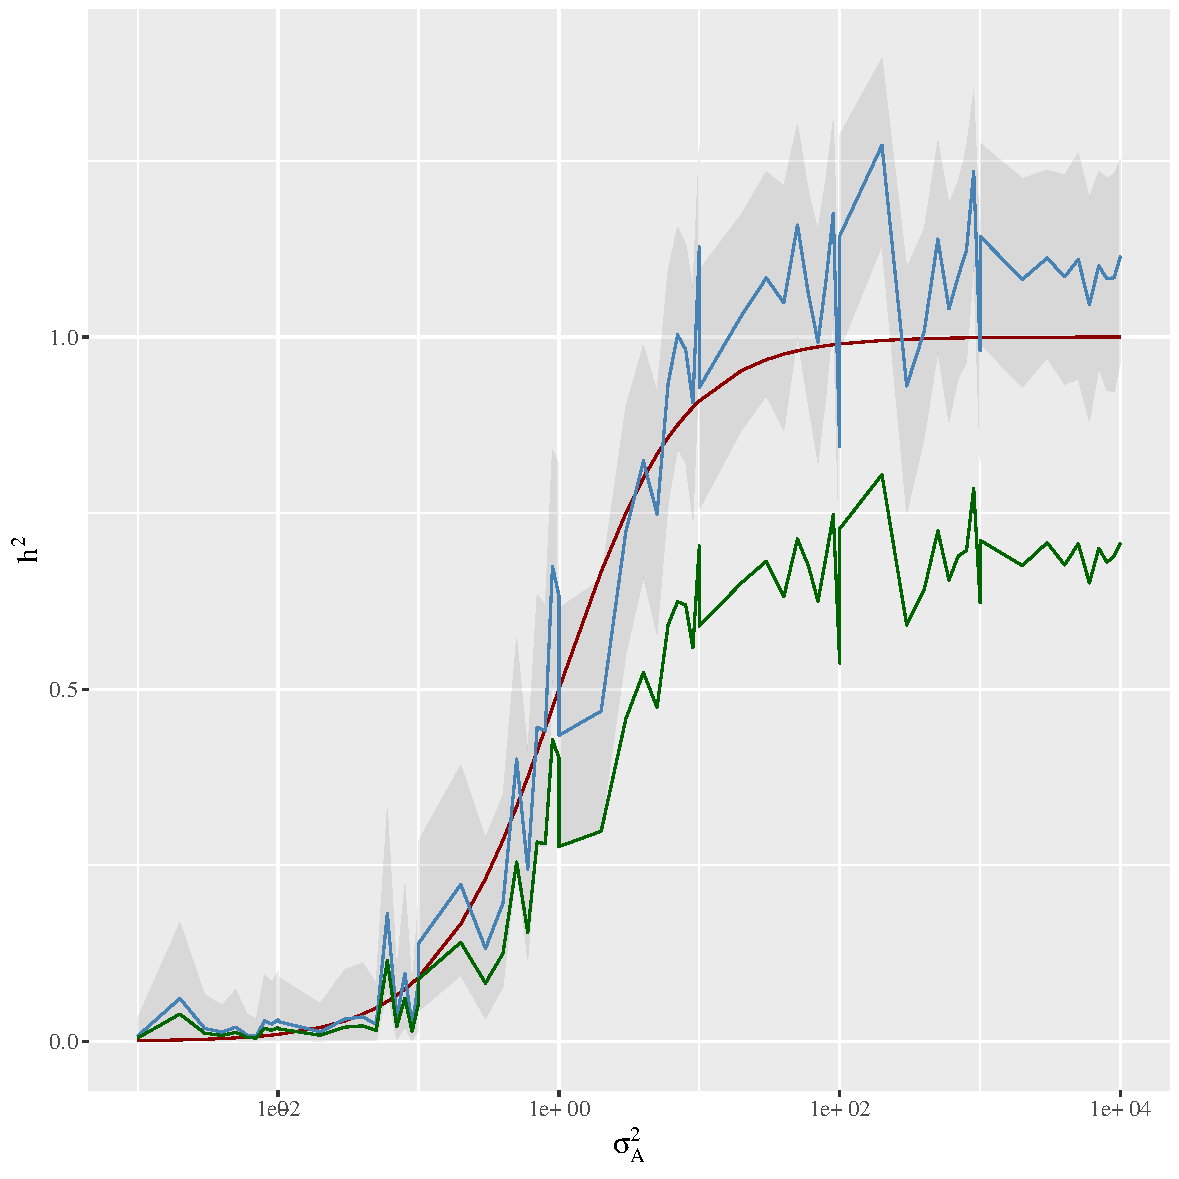
\includegraphics[width=\textwidth]{figures/simulation_deviance_round.pdf}
    \label{fig:simulation_h2_dev:round}
  \end{subfigure}%
  \begin{subfigure}[b]{0.49\textwidth}
    \caption{Binomial dichotomization}
    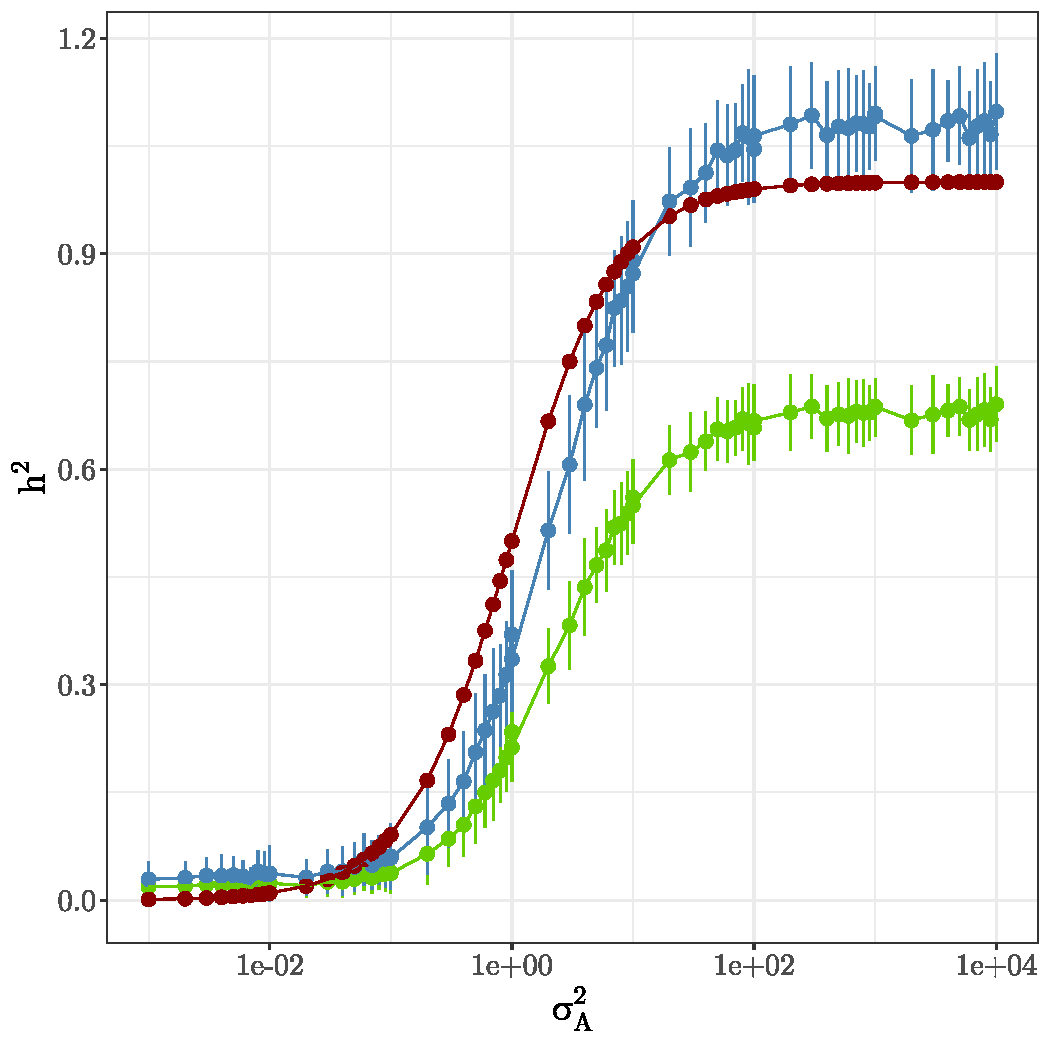
\includegraphics[width=\textwidth]{figures/simulation_deviance_binom.pdf}
    \label{fig:simulation_h2_dev:binom}
  \end{subfigure}
  \begin{subfigure}[b]{0.49\textwidth}
      \caption{Threshold dichotomization for smaller $\sigma^2_A$}
      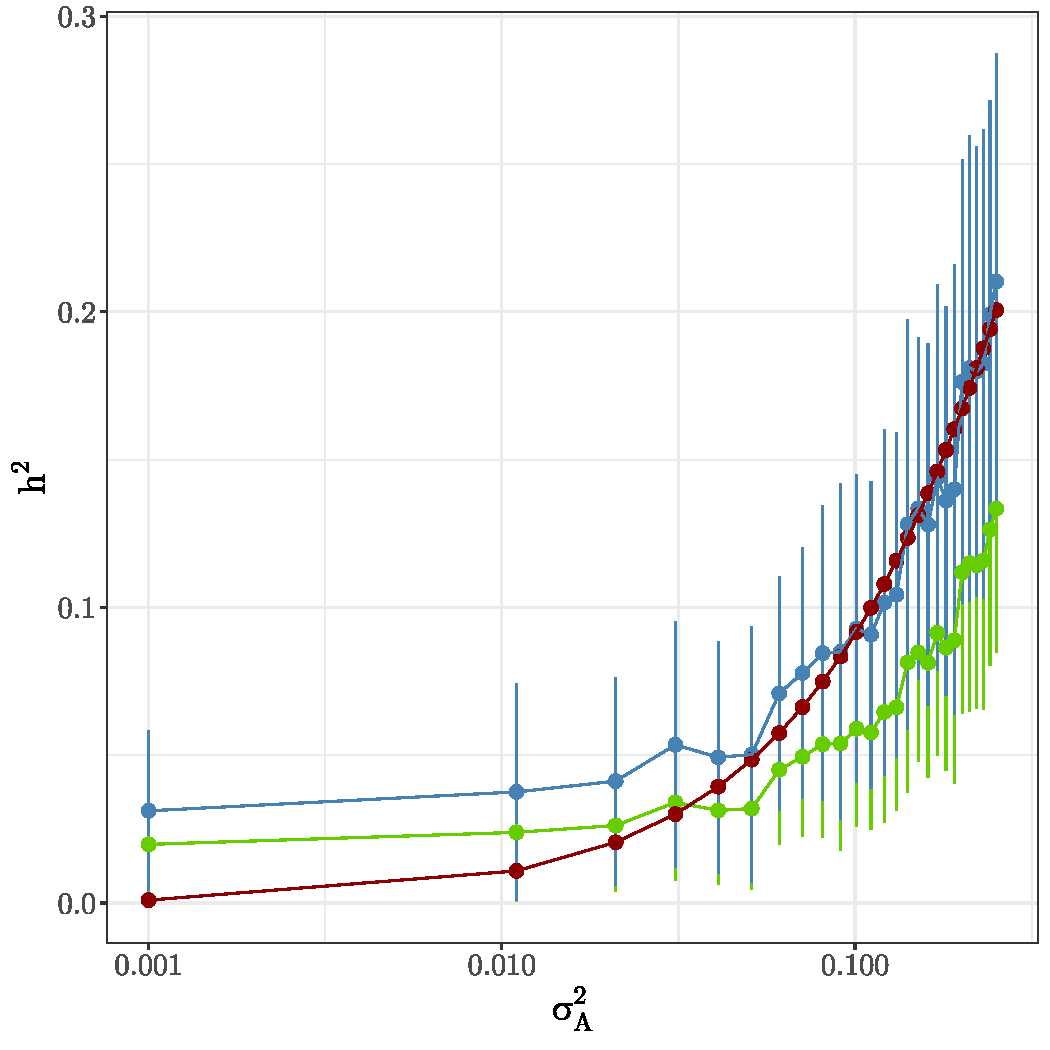
\includegraphics[width=\textwidth]{figures/simulation_deviance_small.pdf}
      \label{fig:simulation_h2_dev:small}
  \end{subfigure}
  \begin{subfigure}[b]{0.49\textwidth}
      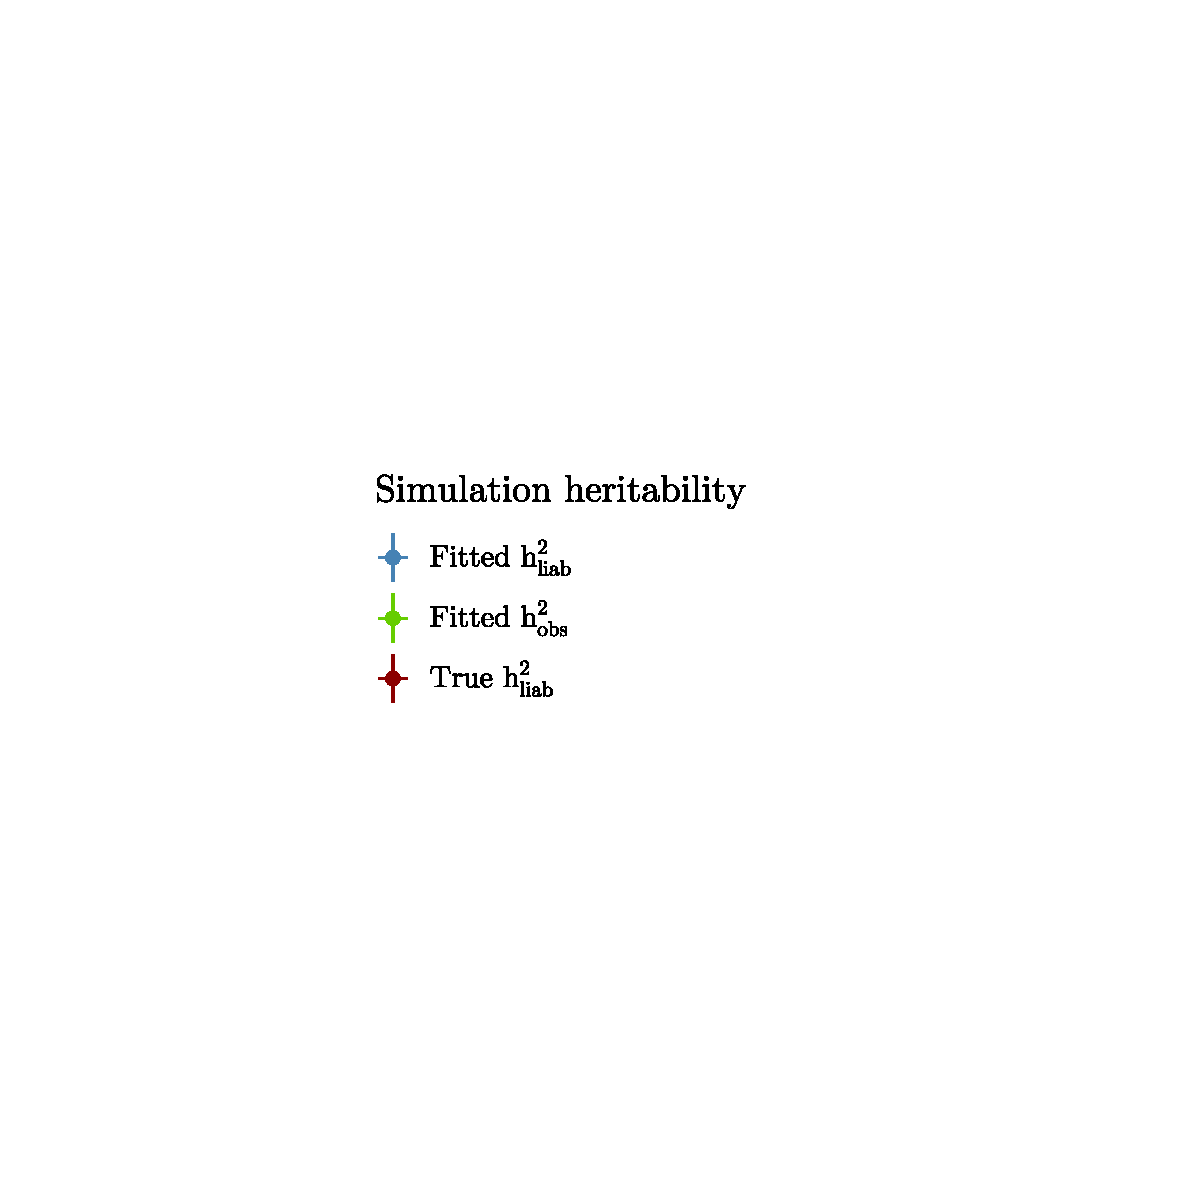
\includegraphics[width=\textwidth, trim={0.7\textwidth} {0.7\textwidth} {0.7\textwidth} {0.7\textwidth},clip]{figures/simulation_deviance_legend.pdf}
  \end{subfigure}
  \caption[Estimated heritability compared to the true value in simulation]{Values of heritabilities for the true, underlying continuous scale in the simulation study (red line), alongside the estimated heritability using a Gaussian model. The green line shows the heritability on the observation scale ($h^2_\text{obs}$) estimated with a Gaussian model using the dichotomized data, whereas the blue line is scaled by the threshold model formula to obtain heritability on the liability scale ($h^2_\text{liab}$). The point shows the mean of 50 runs, with each corresponding line resembling its standard deviation.}
  \label{fig:simulation_h2_dev}
\end{figure}

\subsection{Heritability on different scales}

This section aims to provide an overview of the heritability estimates for its various scales using the simulated data. Initially, we compare the Gaussian and probit models on the liability scale and similarly on the observation scale. Furthermore, we specifically consider the observation-scale heritability of the binomial model ($h^2_\Psi$), where we investigate how changing fixed effects averaging settings may affect $h^2_\Psi$.

The posterior heritability density for the liability and observation scale shows similarities between the Gaussian and probit models for heritability (\autoref{fig:posterior simulation heritability}). The notation and expressions for $h^2_\text{obs}$, $h^2_\text{liab}$, $h^2_\Phi$ and $h^2_\Psi$ are given in \autoref{tab:h2 notation}.
%$h^2_\text{obs}$ is provided from the Gaussian model directly, where $h^2_\text{liab}$ is obtained by multiplying $h^2_\text{obs}$ with the coefficient $p(1-p)/t^2$ \eqref{eq:heritability for threshold model}. Furthermore, $h^2_\Phi$ is the proportion $\hat\sigma^2_A/(\hat\sigma^2_A+\hat\sigma^2_E+1)$ where the estimators are on the latent scale \eqref{eq:link variance h2 phi}, and $h^2_\Psi$ is the back-transformed heritability from the probit model.
Finally, some statistics (the mean, estimated mode, and standard deviation) of the same posteriors are summarized in \autoref{tab:heritability simulation}. Complementary to these results, we report the deviance information criteria for the two models (\autoref{tab:simulation DICs}). In addition to the figures presented here, we refer to \autoref{fig:application gaussian vs binomial} and \autoref{fig:simulatino gaussian vs binomial} in the appendix, providing a grid of density comparisons for the different heritability scales, for the application and simulation data, respectively.

\begin{table}[ht]\centering
% TABLE FROM R: Tue Jun 13 13:48:15 2023 
 \begin{tabular}{lccc}
 \hline
 Model & Mean & Mode & Standard deviation  \\ 
 \hline 

 Gaussian $h^2_\text{obs}$ & 0.131 & 0.117 & 0.049 \\ 
 Probit $h^2_{\Psi}$ & 0.149 & 0.102 & 0.079 \\ 
  & & & \\ 
 Gaussian $h^2_\text{liab}$ & 0.209 & 0.187 & 0.079 \\ 
 Probit $h^2_{\Phi}$ & 0.228 & 0.19 & 0.091 \\ 
 \bottomrule
\end{tabular}


\caption[Heritability means for all scales in simulation]{Heritability estimates for Gaussian and probit models, in the simulation data with $\sigma^2_A=0.5$, showing the mean, mode, and standard deviation. The first two and the last two rows provide heritability comparable to each other. We refer to \autoref{tab:h2 notation} for a reference on how the different scales are computed.}
\label{tab:heritability simulation}
\end{table}

\begin{figure}
    \centering
    \begin{subfigure}{0.49\textwidth}
        \centering
        \caption{Liability scale}
        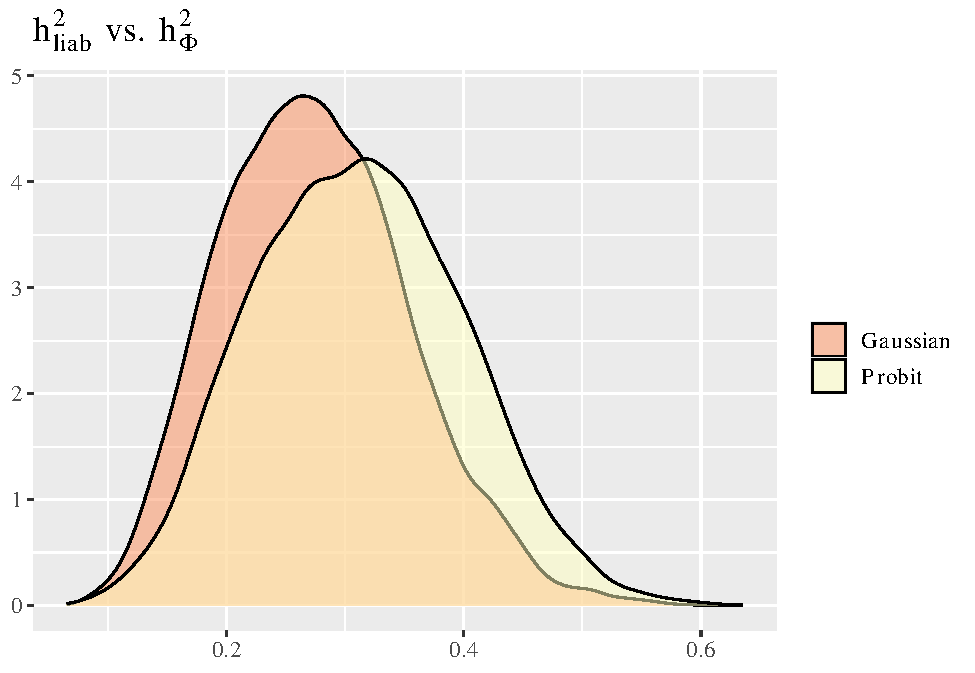
\includegraphics{figures/heritability_simulation_liabscale.pdf}
        \label{fig:posterior simulation heritability:liability}
    \end{subfigure}
    \begin{subfigure}{0.49\textwidth}
        \centering
        \caption{Observation scale}
        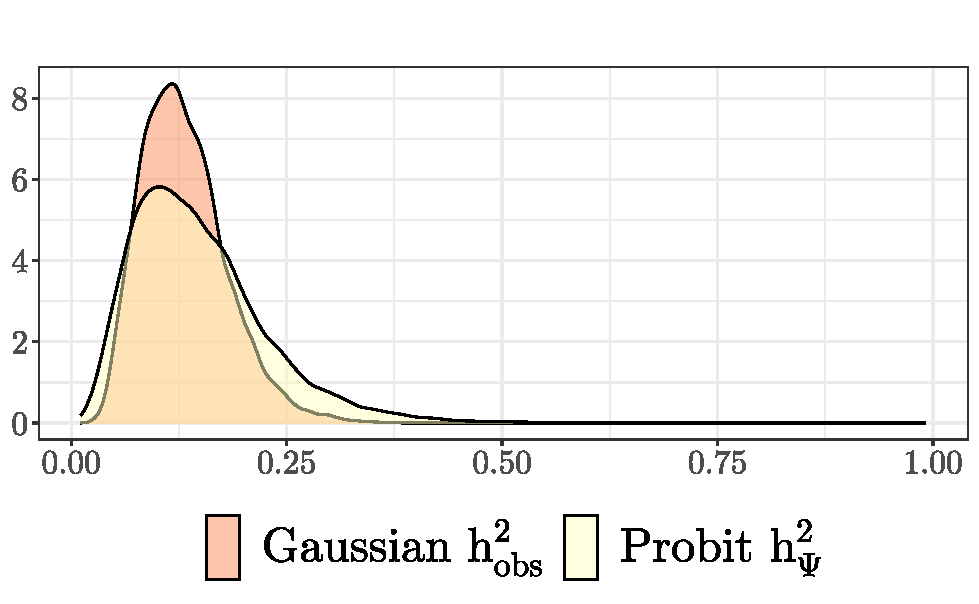
\includegraphics{figures/heritability_simulation_obsscale.pdf}
        \label{fig:posterior simulation heritability:observation}
    \end{subfigure}
    \caption[Heritability density for simulation data]{Posterior liability- and observation-scale densities of heritability for the simulation data.}
    \label{fig:posterior simulation heritability}
\end{figure}

\begin{table}
    \centering
    \begin{tabular}{@{}ll@{}}
    \toprule
        Model           & DIC (Simulation data) \\ \midrule
        Binomial probit & 1180.620 \\
        Gaussian        & 1215.321\\
        \bottomrule
    \end{tabular}
    \caption[DIC for simulation data]{Deviance information criteria (DIC) for the two model fits, for the simulation data, with $\sigma^2_A=0.5$ fixed.}
    \label{tab:simulation DICs}
\end{table}

\subsubsection{Observation scale from probit model}
In the framework from \textcite{de2016general}, there are several parameter settings for computing observation scale heritability $h^2_\Psi$ from binary data, whose difference is described in the methods chapter (\autoref{sec:method:qgglmm settings}). As such, we first investigate to what extent the heritability densities differ from each other. The resulting posteriors for $h^2_\Psi$ are provided in \autoref{fig:qgglmm simulation} for the simulation data, showing little difference for a small $\sigma^2_A=0.1$, although larger deviations for a larger $\sigma^2_A$. In addition to these posteriors, we show the runtime for computing $10,000$ samples in \autoref{tab:h2psi runtime}.

\begin{table}
% Called function at: Wed Apr 26 14:28:32 2023 
% Entering `new.h2.transf` (Bayesian sampling)
% DEBUG: Entering sampling for loop
% DEBUG: Entering transposing loop
% Done after 3.327576 minutes. Entering same function without the Bayesian stuff.
% Done after 0.1665074 minutes. Now without averaging:Done after 0.06656845 minutes.
% Saving to disk...
% [1] 0
    \centering
    \begin{tabular}{@{}lr@{}}
    \toprule
    Estimate & Runtime \\ \midrule
    $h^2_\Psi$ Bayesian & $26$ sec \\
    $h^2_\Psi$ Frequentist & $11$ sec \\
    $h^2_\Psi$ No averaging & $4$ sec \\
    \bottomrule
    \end{tabular}
    \caption[Runtime of computing $h^2_\Psi$]{Runtime of computing $10,000$ samples of $h^2_\Psi$ in seconds for the three methods provided by the \texttt{QGglmm} package, in simulation data with $900$ observations.}
    \label{tab:h2psi runtime}
\end{table}


% <<<<< QGglmm comparisons
\begin{figure}
    \centering
    \begin{subfigure}[b]{0.49\textwidth}
        \caption{$\sigma^2_A=0.1$}
        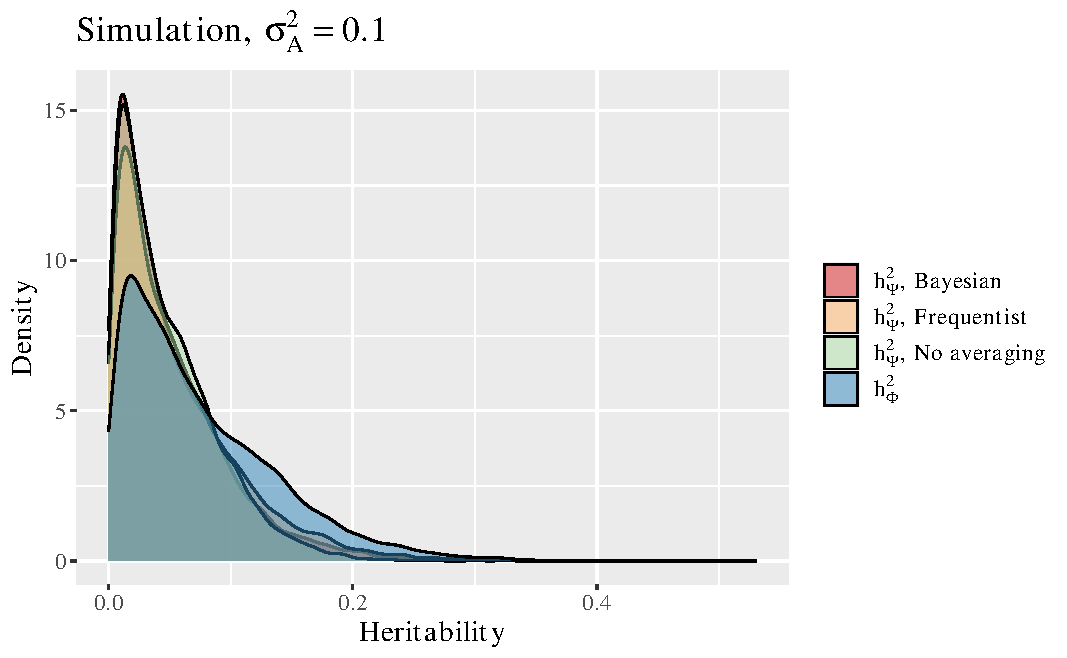
\includegraphics[width=\textwidth]{figures/qgglmm-comparison-simulationva0.1.pdf}     
    \end{subfigure}
    \begin{subfigure}[b]{0.49\textwidth}
        \caption{$\sigma^2_A=1$}
        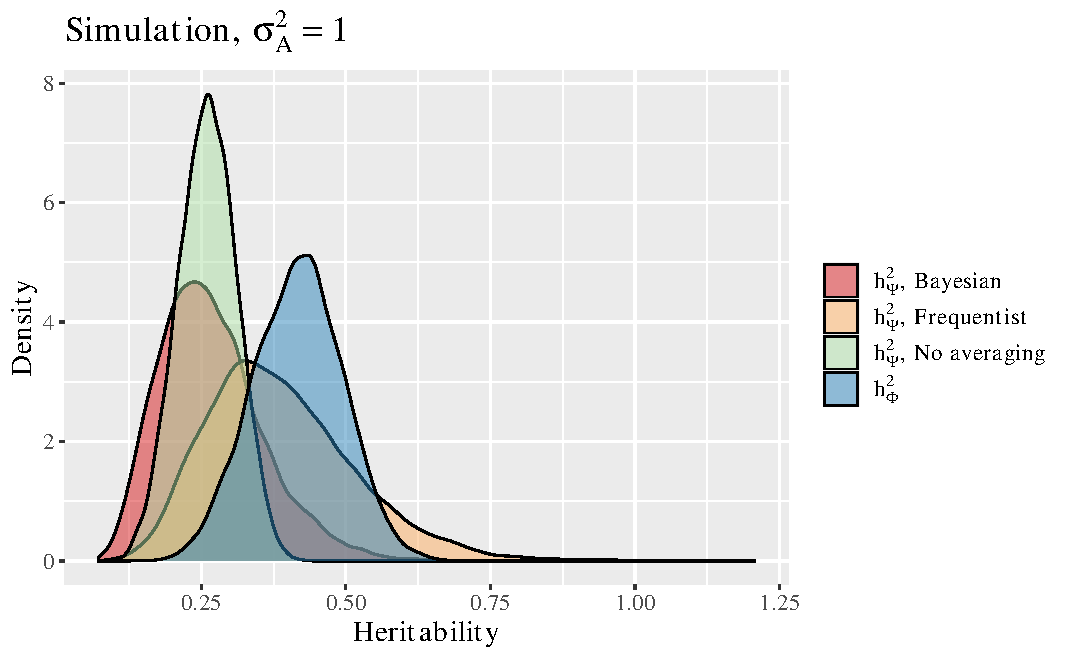
\includegraphics[width=\textwidth]{figures/qgglmm-comparison-simulationva1.pdf}\label{fig:qgglmm simulation:bigvA}
    \end{subfigure}
    \begin{subfigure}[b]{0.25\textwidth}
    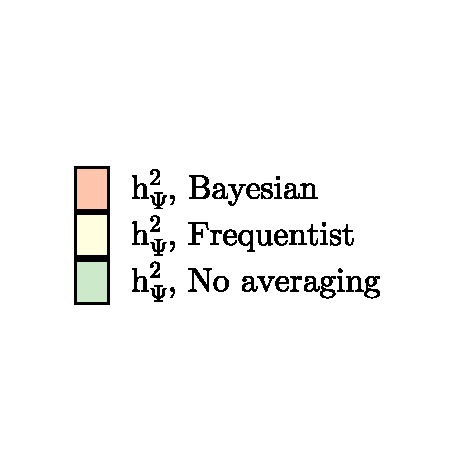
\includegraphics[width=\textwidth, trim={0.3\textwidth} {0.3\textwidth} {0.3\textwidth} {0.3\textwidth},clip]{figures/qgglmm-comparison-simulation-legend.pdf}
    \end{subfigure}
    \caption[$h^2_\Psi$ on simulations, with varying parameter settings]{Estimated posterior heritability for the different back-transformations techniques, for a binomial probit model to simulations with small variance ($\sigma^2_A=0.1$) and a simulation with larger variance ($\sigma^2_A=1$), respectively.}
    \label{fig:qgglmm simulation}
\end{figure}


% >>>>> QGglmm comparisons

%In the application case, all three discussed methods for computing $h^2_\Psi$ are very similar.
% Now, we want to see what the Gaussian model looks like compared to the other methods. The notation here is described in \autoref{tab:h2 notation}. %% ???
\subsection{Robustness tests}
Lastly, we present some results exploring the robustness of the models, namely by introducing fixed effects and overdispersion. \autoref{fig:fixed effects sim deviance gaussian model} illustrates how the heritability of the Gaussian model, once transformed to its liability scale, is relative to the theoretical value for varying values of $\sigma^2_A$. In this context, the theoretical value includes fixed effects variance in the denominator, \autocite{nakagawa2013general}
\begin{equation}
    h^2_\text{liab} = \frac{\sigma^2_A}{\sigma^2_A + \sigma^2_E + \beta_\text{sex}^2\sigma^2_{\text{sex}}} \ .
\end{equation}

The plot is similar to \autoref{fig:simulation_h2_dev}, although the subplots differ in the magnitude of the fixed effect term rather than different dichotomization methods. We can also see a significant deviation between the estimated and true $h^2_\text{liab}$ for the case of fixed effects. Additionally, we provide the posterior density of heritability when including fixed effects to assess differences quantitatively (\autoref{fig:fixedeffects probit vs gaussian}). The plot shows the posterior heritabilities for a Gaussian and a probit model fitted on simulation data where $\beta_{\text{sex}}=10$, $\sigma^2_E=1$, and varying $\sigma^2_A$ and $\hat p$. It seems like the estimate from the Gaussian and probit models differ more in the presence of fixed effects.
The second robustness factor examined is overdispersion. The heritability of the resulting models for varying $\sigma^2_E$ are shown in \autoref{fig:overdisperion plots}, where generally all models seem to produce similar posterior heritability estimates.

\begin{figure}
    \centering
    \begin{subfigure}{0.49\textwidth}
    \caption{}
        % \caption{$\beta_\text{sex}=10$, unbalanced $p = 0.1$ for each simulation.}
        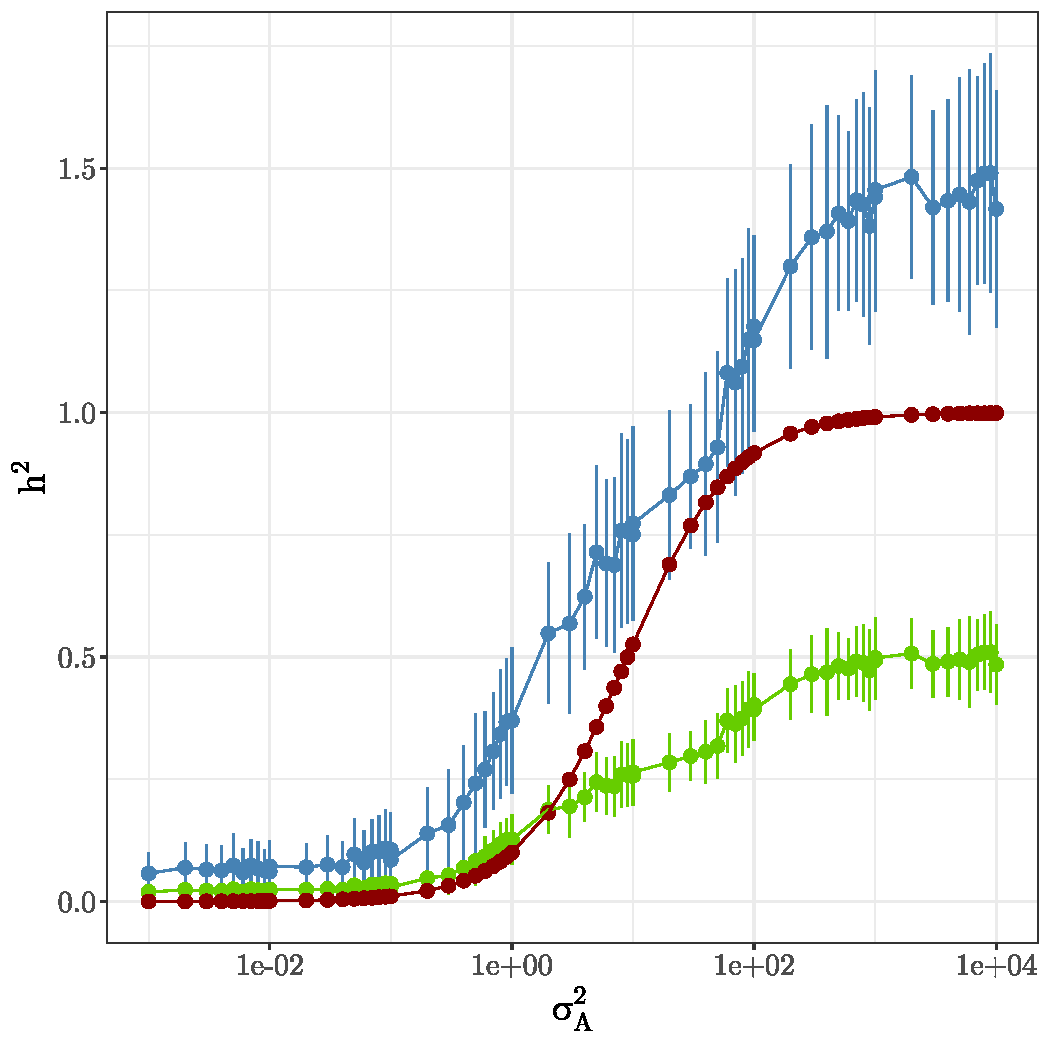
\includegraphics[width=\linewidth]{figures/simulation_deviance_fixedeffects_beta10_unbalanced.pdf}
    \end{subfigure}
    \begin{subfigure}{0.49\textwidth}
    \caption{}
        % \caption{$\beta_\text{sex}=10$, balanced $p\in [0.48, 0.52]$ with 95\% confidence.}
        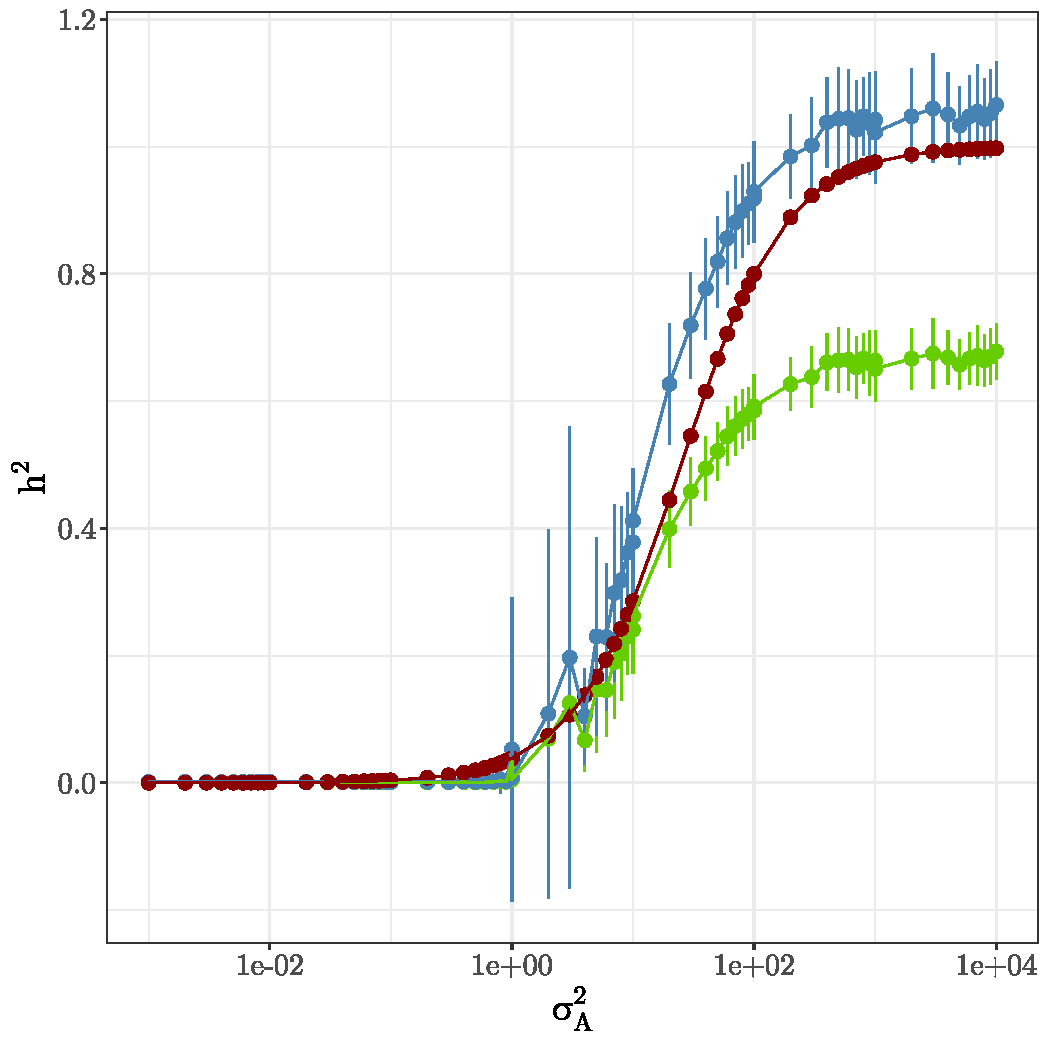
\includegraphics[width=\linewidth]{figures/simulation_deviance_fixedeffects_beta10.pdf}
    \end{subfigure}
        \begin{subfigure}{0.49\textwidth}
        \caption{}
        % \caption{$\beta_\text{sex}=100$, balanced $p \in [0.49, 0.51]$ with 95\% confidence.}
        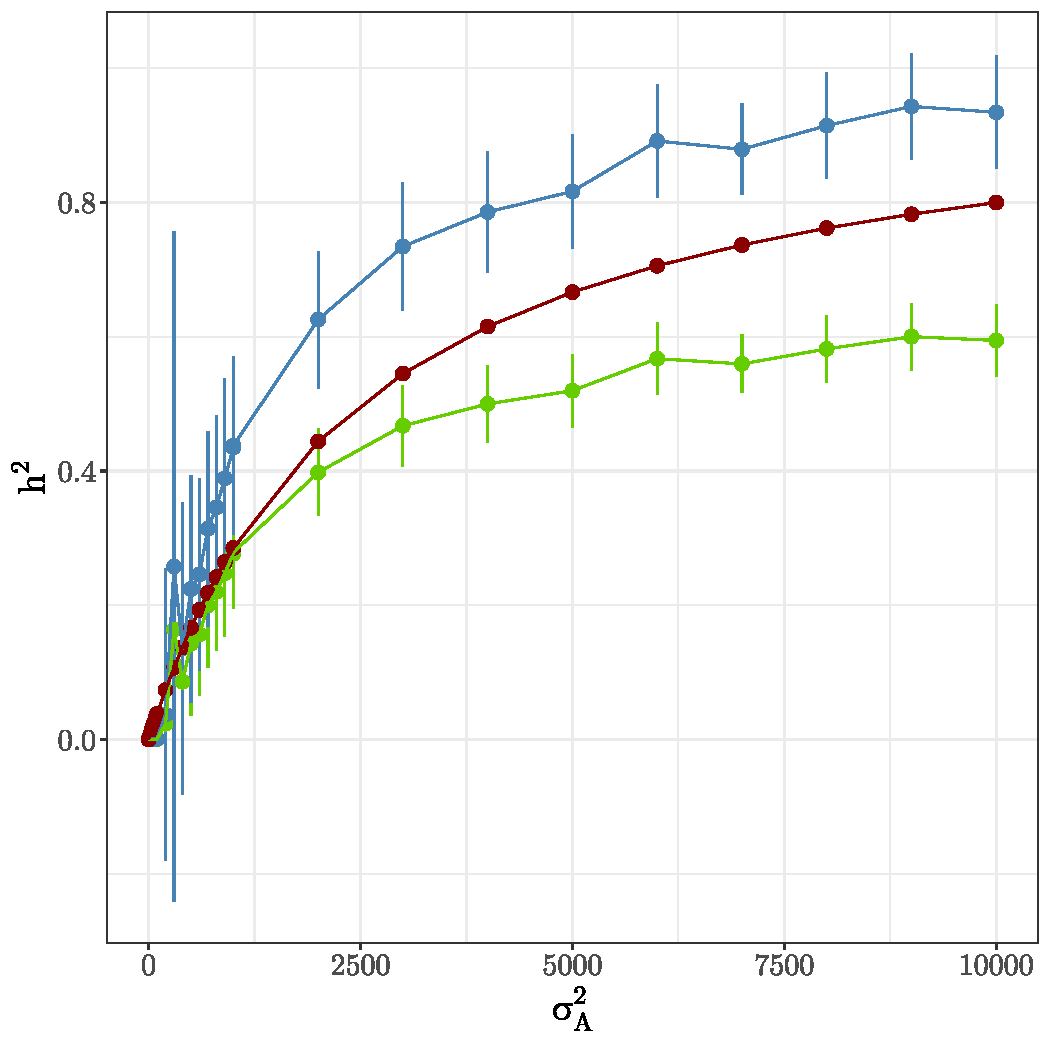
\includegraphics[width=\linewidth]{figures/simulation_deviance_fixedeffects_beta100.pdf}
    \end{subfigure}
    \begin{subfigure}{0.49\textwidth}
        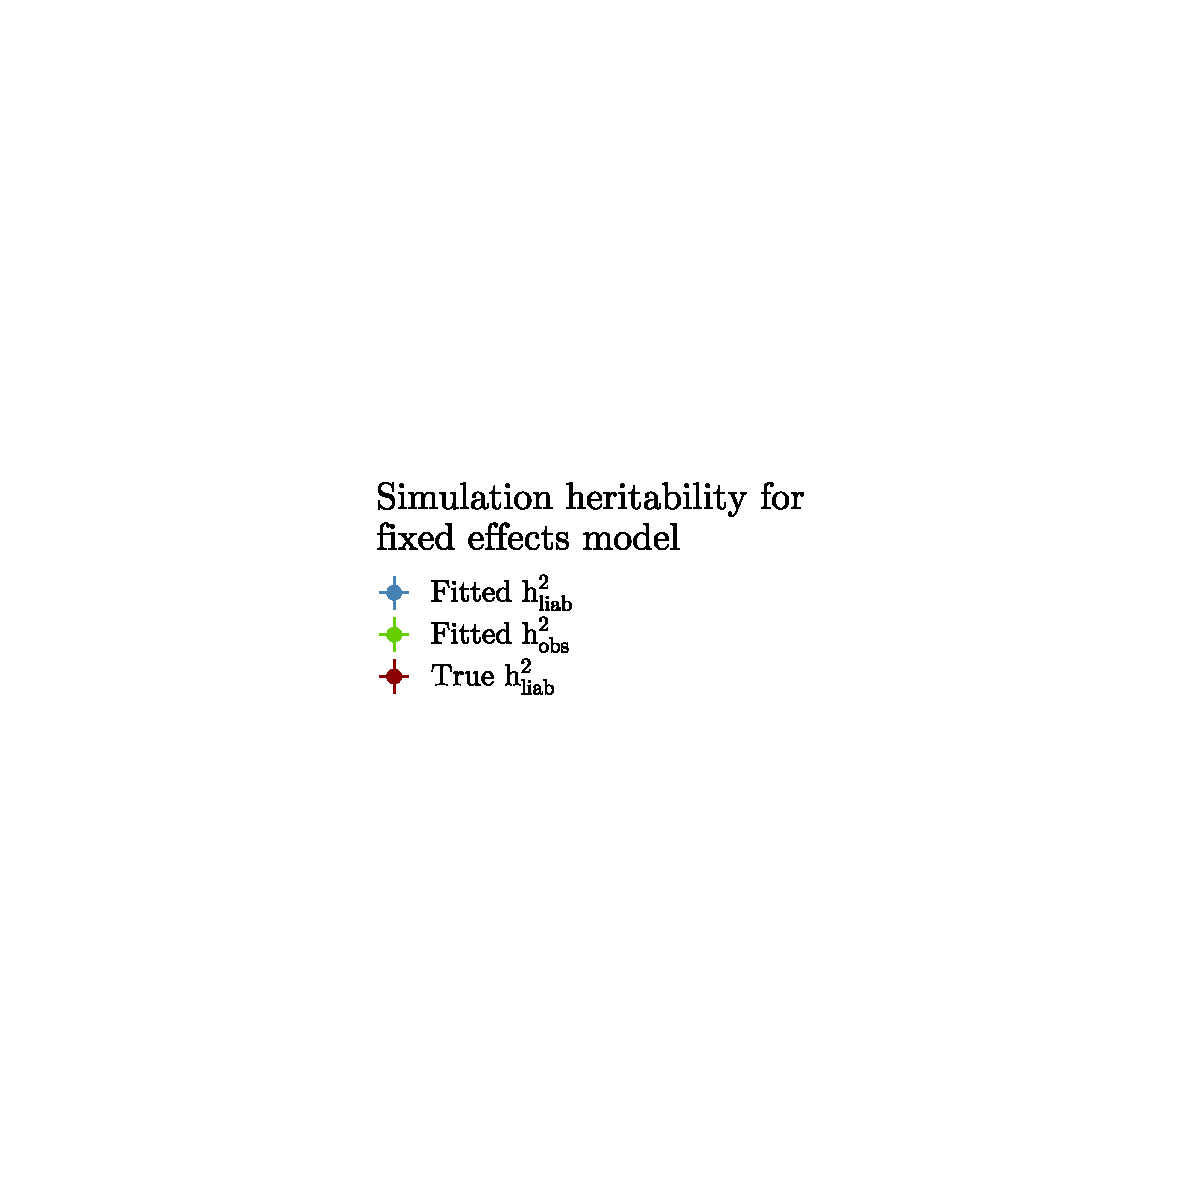
\includegraphics[width=\linewidth, trim={0.7\textwidth} {0.7\textwidth} {0.7\textwidth} {0.7\textwidth},clip]{figures/simulation_deviance_fixedeffects_legend.pdf}
    \end{subfigure}
    \caption[Estimated $h^2_\text{liab}$ compared to true value for fixed effects models]{Estimates for heritability with a Gaussian model including fixed effects. The red line shows the true heritability on the liability scale and includes fixed effects variance as part of phenotypic variance. Subfigure \textbf{(a)} shows the results for an unbalanced $\hat p=0.1$ and $\beta_\text{sex}=10$, whereas the phenotypic mean is balanced in the other subfigures. Furthermore, subfigure \textbf{(b)} demonstrate $\beta_\text{sex}=10$ and \textbf{(c)} with $\beta_\text{sex}=100$. The points show the mean over 50 runs with each corresponding line resembling its standard deviation.}
    \label{fig:fixed effects sim deviance gaussian model}
\end{figure}

\begin{figure}
    \centering
    \begin{subfigure}{0.49\textwidth}
    \caption{$\beta=10$, $\sigma^2_A=10$, $\sigma^2_E=1$, $\hat p=0.1$}
    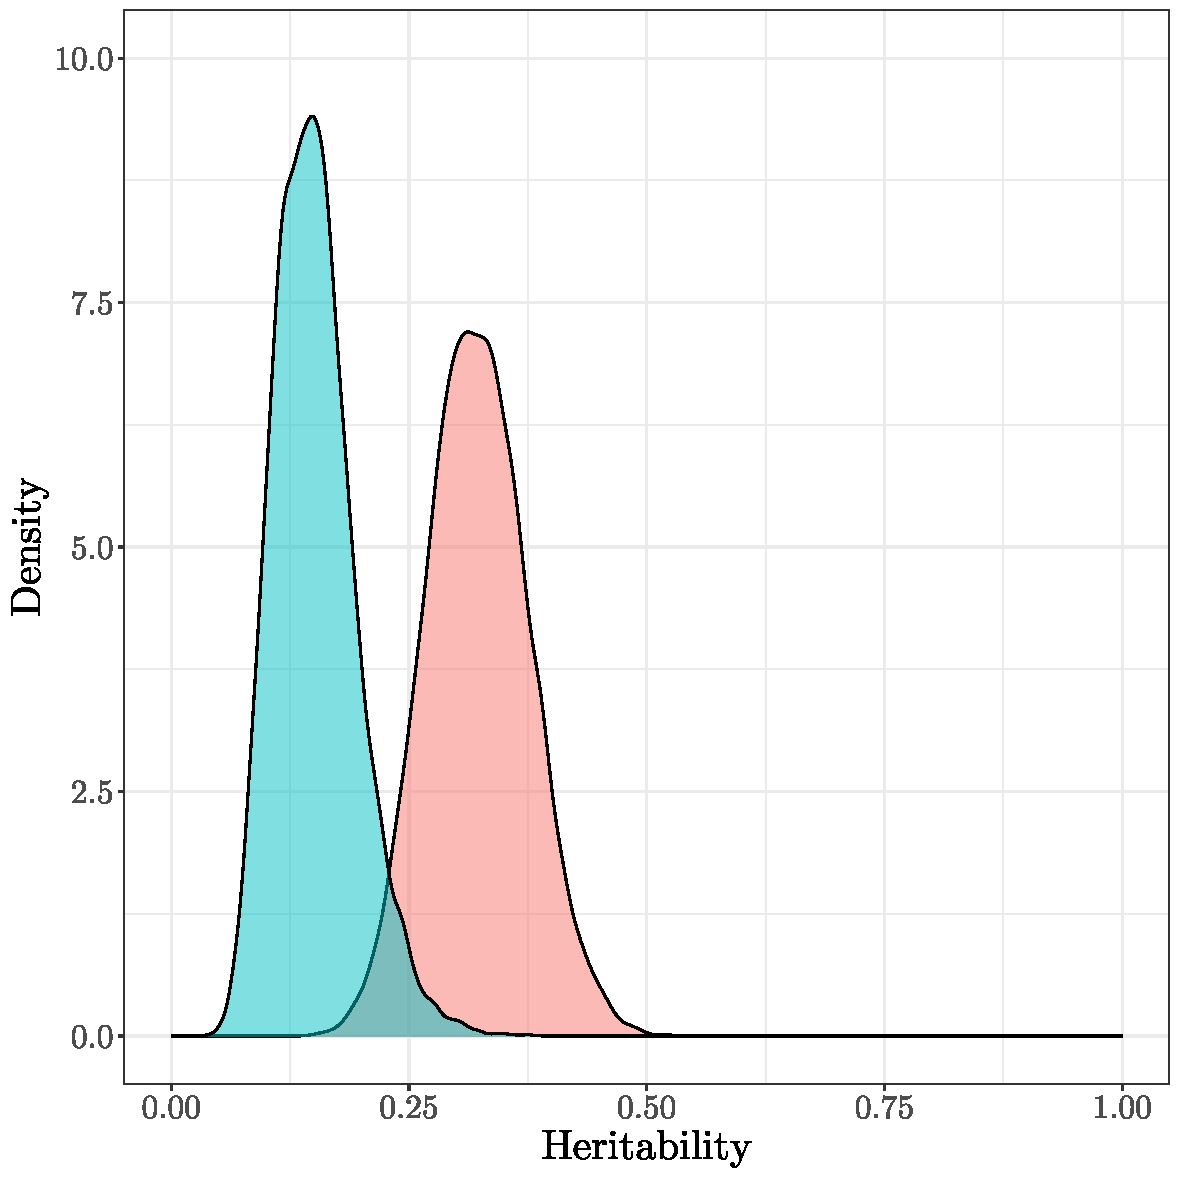
\includegraphics[width=\textwidth]{figures/fixedeffects_gaussian_probit_sA10_p_1.pdf}
    \label{fig:fixedeffects probit vs gaussian:lVAlP}
    \end{subfigure}
    \begin{subfigure}{0.49\textwidth}
    \caption{$\beta=10$, $\sigma^2_A=10$, $\sigma^2_E=1$, $\hat p=0.5$}
    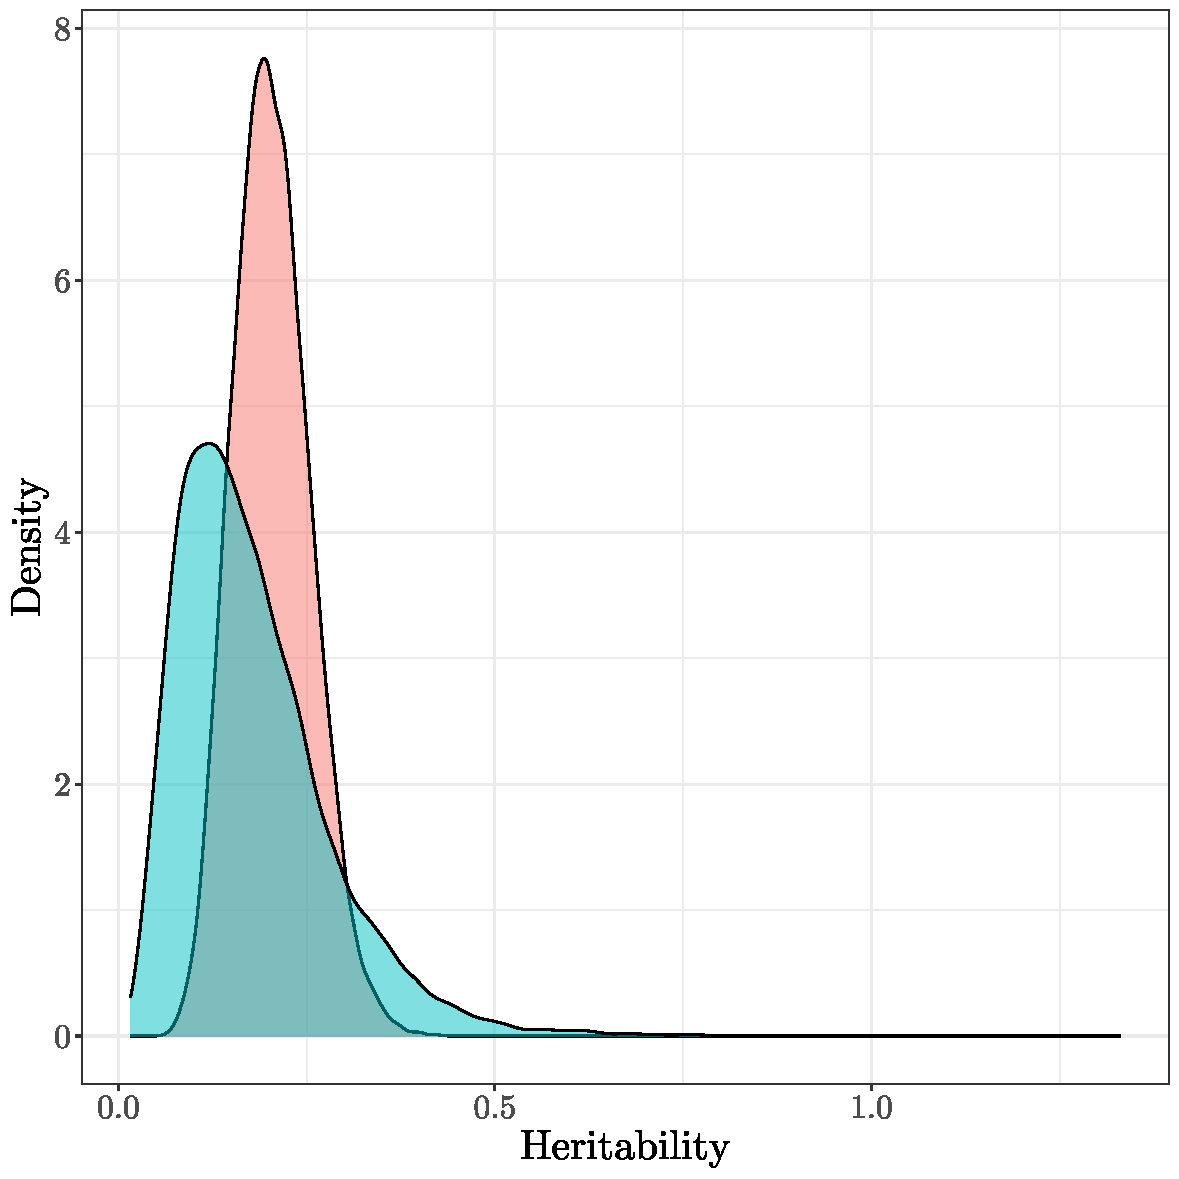
\includegraphics[width=\textwidth]{figures/fixedeffects_gaussian_probit_sA10_p_5.pdf}
    \label{fig:fixedeffects probit vs gaussian:lVAhP}
    \end{subfigure}
    \begin{subfigure}{0.49\textwidth}
    \caption{$\beta=10$, $\sigma^2_A=500$, $\sigma^2_E=1$, $\hat p=0.1$}
    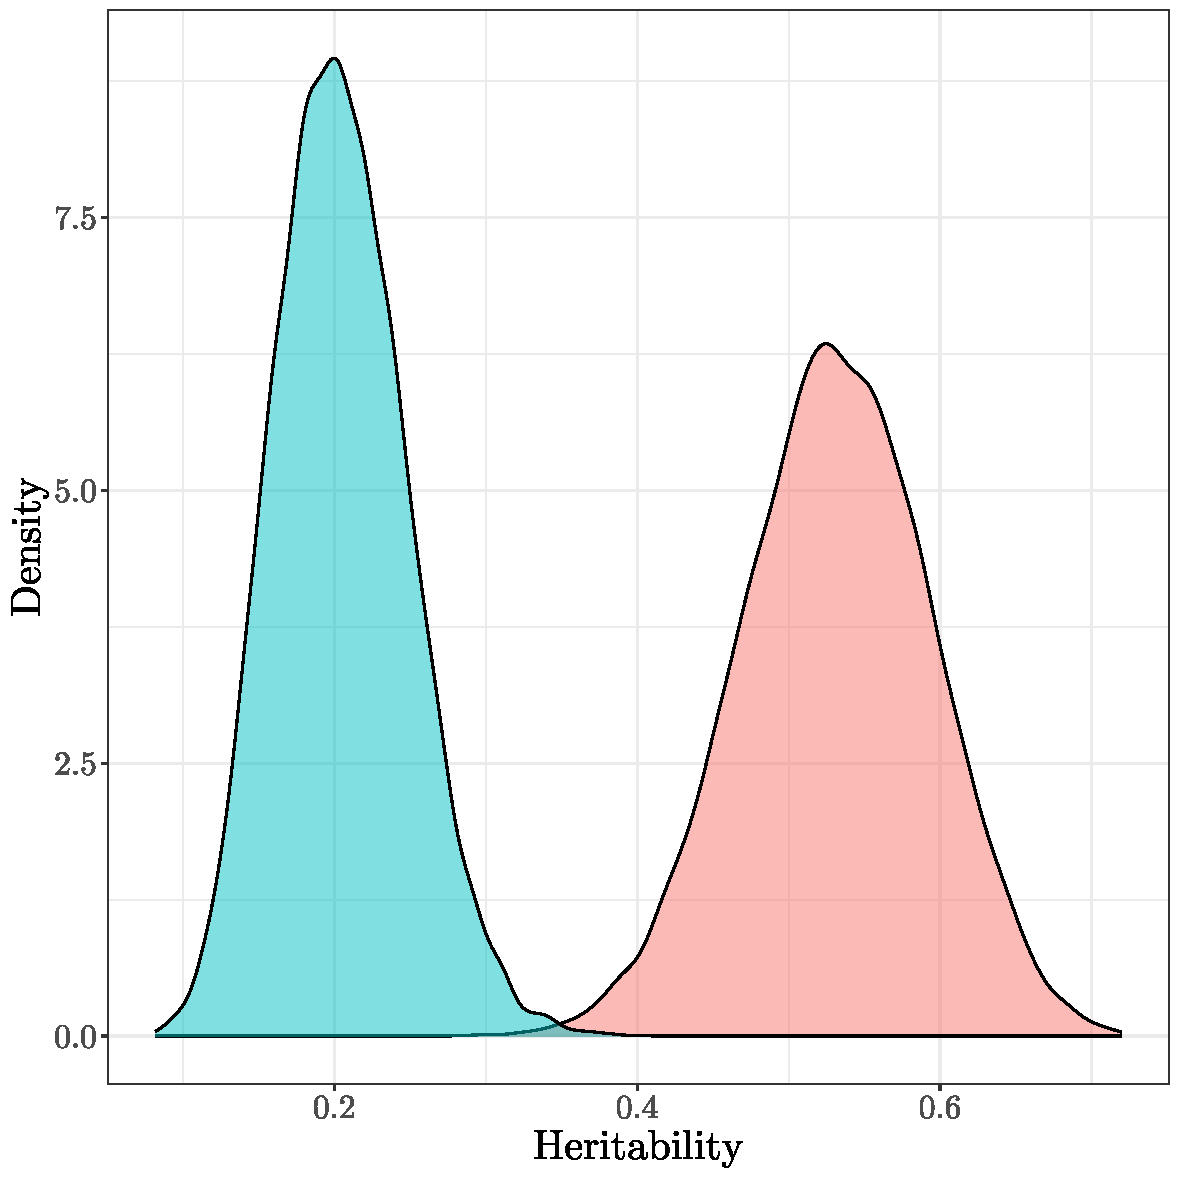
\includegraphics[width=\textwidth]{figures/fixedeffects_gaussian_probit_sA500_p_1.pdf}
    \label{fig:fixedeffects probit vs gaussian:hVAlP}
    \end{subfigure}
    \begin{subfigure}{0.49\textwidth}
    \caption{$\beta=10$, $\sigma^2_A=500$, $\sigma^2_E=1$, $\hat p=0.5$}
    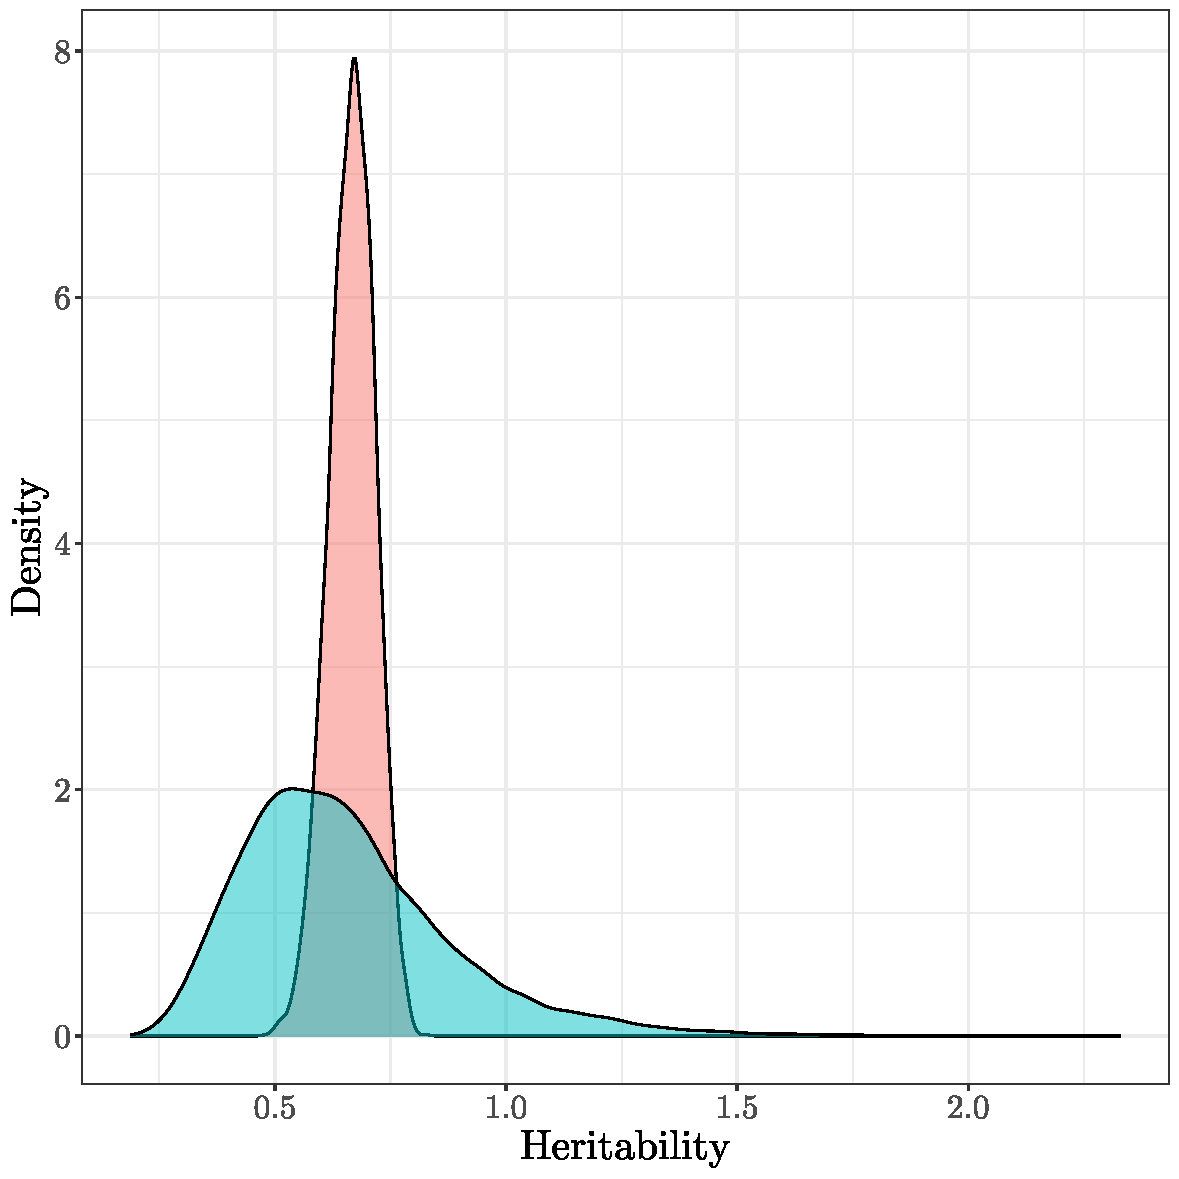
\includegraphics[width=\textwidth]{figures/fixedeffects_gaussian_probit_sA500_p_5.pdf}
    \label{fig:fixedeffects probit vs gaussian:hVAhP}
    \end{subfigure}
    \begin{subfigure}{0.6\textwidth}
    
\includegraphics[width=\textwidth]{figures/fixedeffects_gaussian_probit_legend.pdf}
    \end{subfigure}
    \caption[$h^2$ for fixed effects simulation models]{Posterior heritability for simulations with fixed effects on observation-scale. The first column shows the results with an unbalanced trait, $p=0.1$, and the other column for a balanced trait $p=0.5$. Furthermore, the first row show densities where $\sigma^2_A=10$, and the second row when $\sigma^2_A=500$.}
    \label{fig:fixedeffects probit vs gaussian}
\end{figure}
% \begin{figure}
%     \centering
%     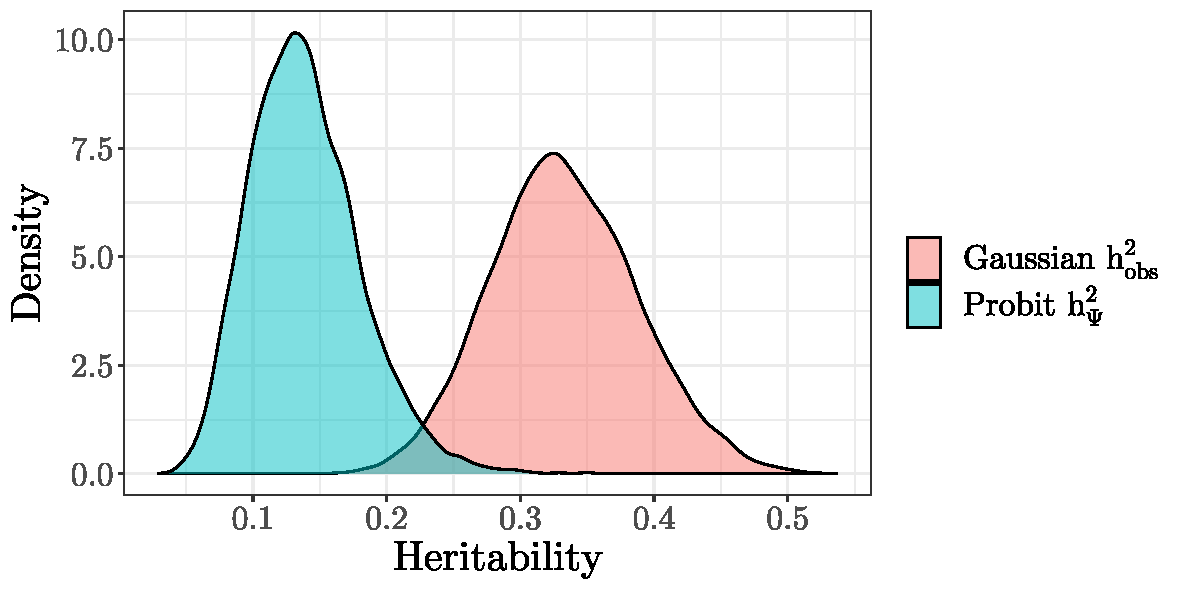
\includegraphics{figures/density-fixed/fixedeffects_gaussian_probit_sA10_p_1_wide.pdf}
%     \caption[$h^2$ density on observation scale for fixed effects model]{A comparison between the posterior heritability on observation-scale for a Gaussian (red) and binomial probit model (blue), the latter of which is back-transformed by \autoref{alg:qgglmm-probit}. The dashed, dark red line shows the theoretical observation-scale heritability in the simulation model. That is, threshold-scaled $h^2_\text{obs}$ for the corresponding $h^2_\text{liab}=\sigma^2_A/(\sigma^2_A+\sigma^2_E+\Var{\beta_\text{sex}\bf x_{\text{sex}}})$. In this particular case, $\beta=10$, $\sigma^2_A=10$ and $\sigma^2_E=1$. }
%     \label{fig:fixedeffects probit vs gaussian vs true}
% \end{figure}


\begin{figure}[H]
    \centering
    \begin{subfigure}{0.49\textwidth}
        \caption{$\sigma^2_A=0.5$, $\sigma^2_E=2$}
        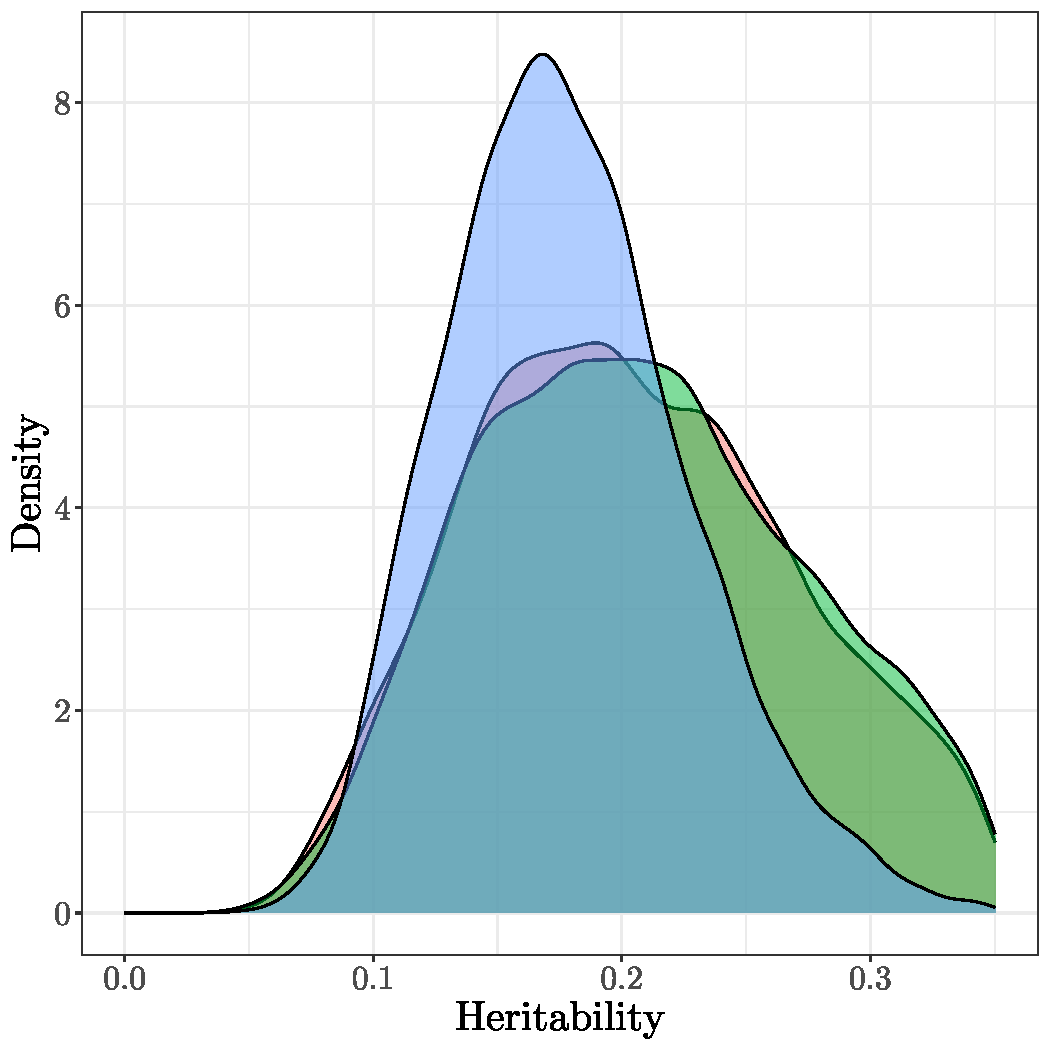
\includegraphics[width=\linewidth]{figures/overdispersion_vE-vA_2-0.5.pdf}
    \end{subfigure}
    \begin{subfigure}{0.49\textwidth}
        \caption{$\sigma^2_A=0.5$, $\sigma^2_E=5$}
        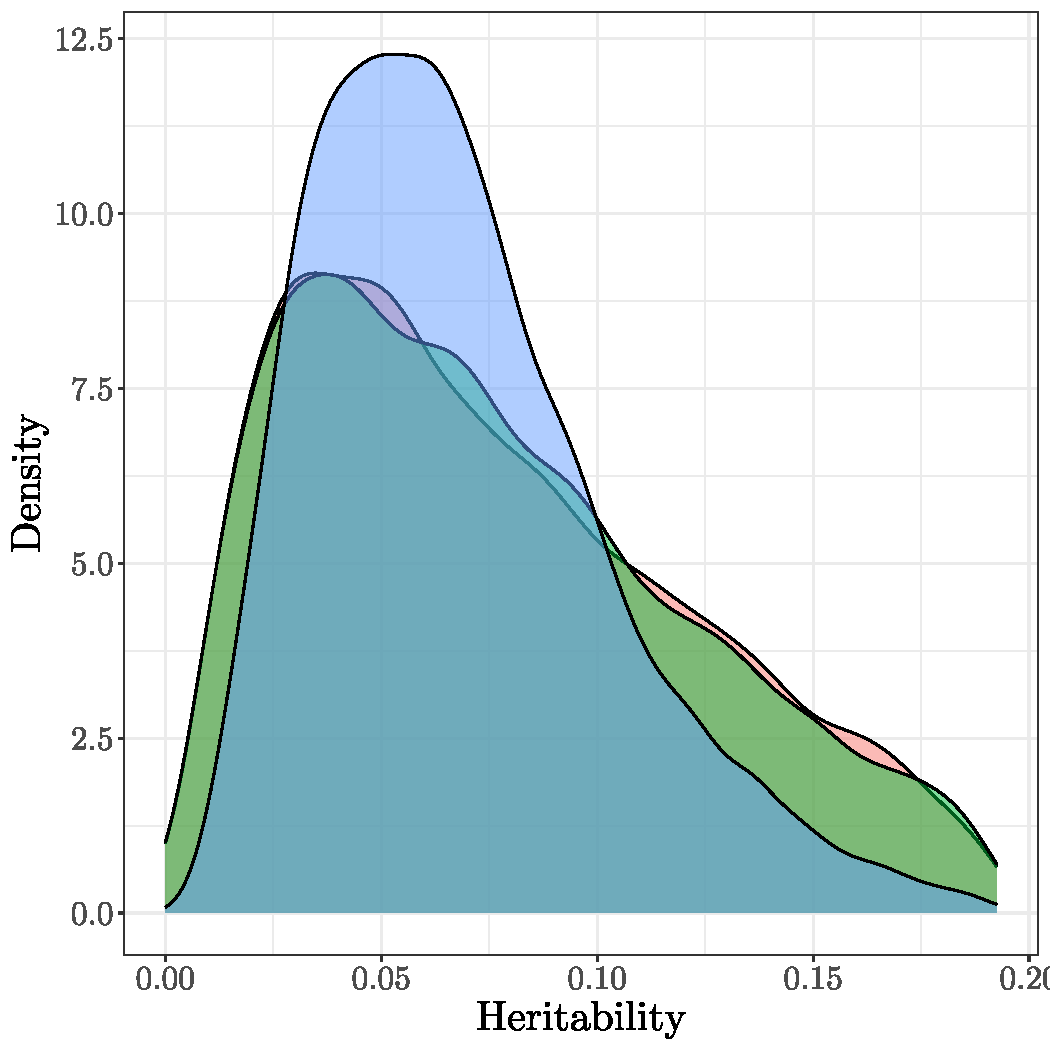
\includegraphics[width=\linewidth]{figures/overdispersion_vE-vA_5-0.5.pdf}
    \end{subfigure}
    \begin{subfigure}{0.49\textwidth}
        \caption{$\sigma^2_A=0.5$, $\sigma^2_E=10$}
        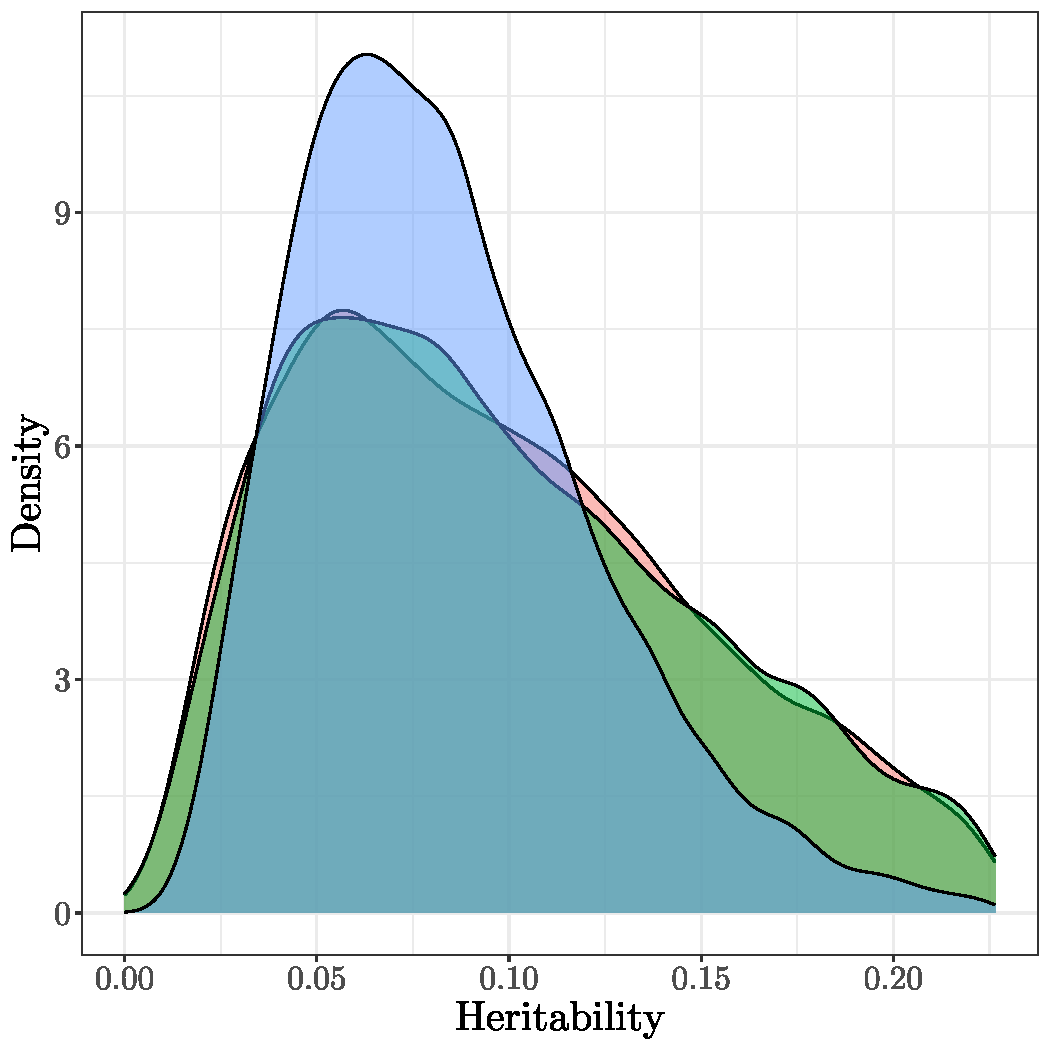
\includegraphics[width=\linewidth]{figures/overdispersion_vE-vA_10-0.5.pdf}
    \end{subfigure}
    \begin{subfigure}{0.49\textwidth}
        \caption{$\sigma^2_A=10$, $\sigma^2_E=10$}
        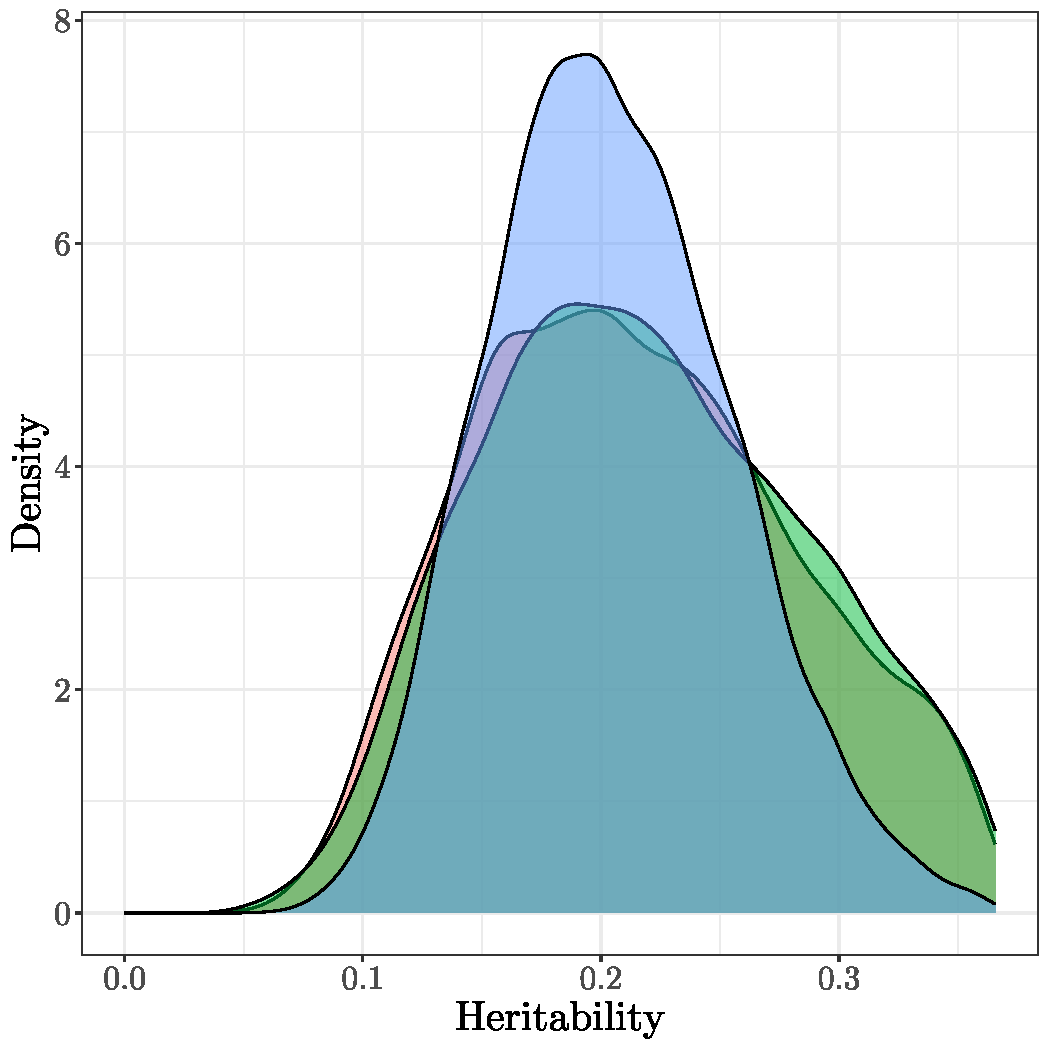
\includegraphics[width=\linewidth]{figures/overdispersion_vE-vA_10-10.pdf}
    \end{subfigure}
    \begin{subfigure}{\textwidth}
        
\includegraphics[width=\textwidth]{figures/overdisperions_legend.pdf}
    \end{subfigure}
    \caption[Posterior with and without overdispersion (simulation data)]{A comparison between two probit models and a Gaussian model fitted with the simulation data. One of the probit models has an additional random iid effect to account for overdispersion, whereas the other does not have the random iid effect. The heritability densities are shown for varying $\sigma^2_A$ and $\sigma^2_E$. %The dashed, dark red line resembles the true observation scale heritability for the simulation.
    }
    \label{fig:overdisperion plots}
\end{figure}


\section{Application study}

\subsection{Heritability on different scales}
Replicating the method in the previous section, we present the heritability estimates for the application data. They are provided in \autoref{fig:posterior application heritability} and \autoref{tab:heritability application}, showing similarities between the heritability of the Gaussian and probit models on the respective scales. Similarly to the simulation case, we employ the different parameter settings in the algorithm for observation-scale heritability from the probit model, yielding \autoref{fig:qgglmm application}.
 
\begin{table}[ht]\centering
% TABLE FROM R: Tue Jun 13 13:48:14 2023 
 \begin{tabular}{lccc}
 \hline
 Model & Mean & Mode & Standard deviation  \\ 
 \hline 

 Gaussian $h^2_\text{obs}$ & 0.034 & 0.025 & 0.018 \\ 
 Probit $h^2_{\Psi}$ & 0.03 & 0.02 & 0.016 \\ 
  & & & \\ 
 Gaussian $h^2_\text{liab}$ & 0.062 & 0.046 & 0.032 \\ 
 Probit $h^2_{\Phi}$ & 0.055 & 0.042 & 0.027 \\ 
 \bottomrule
\end{tabular}

\caption[Heritability means for all scales in application data]{Heritability estimates for the Gaussian and probit models, in the application data, showing the mean, mode, and standard deviation. The first and last two rows provide heritability comparable to one another. We refer to \autoref{tab:h2 notation} for a reference on how the different scales are computed.}
\label{tab:heritability application}
\end{table}

\begin{figure}
    \centering
    \begin{subfigure}{0.49\textwidth}
        \centering
        \caption{Liability scale}
        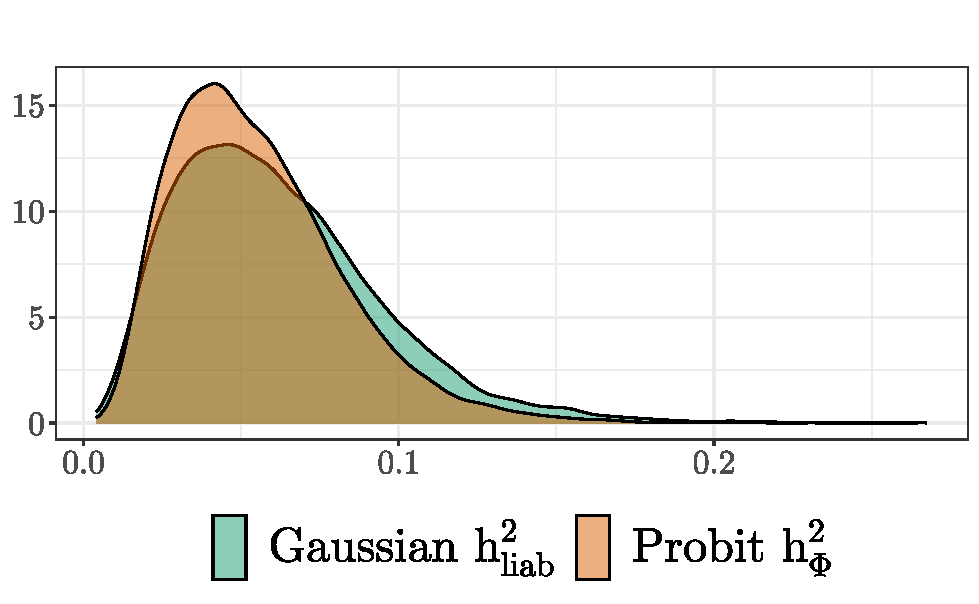
\includegraphics{figures/heritability_application_liabscale.pdf}
        \label{fig:posterior application heritability:liability}
    \end{subfigure}
    \begin{subfigure}{0.49\textwidth}
        \centering
        \caption{Observation scale}
        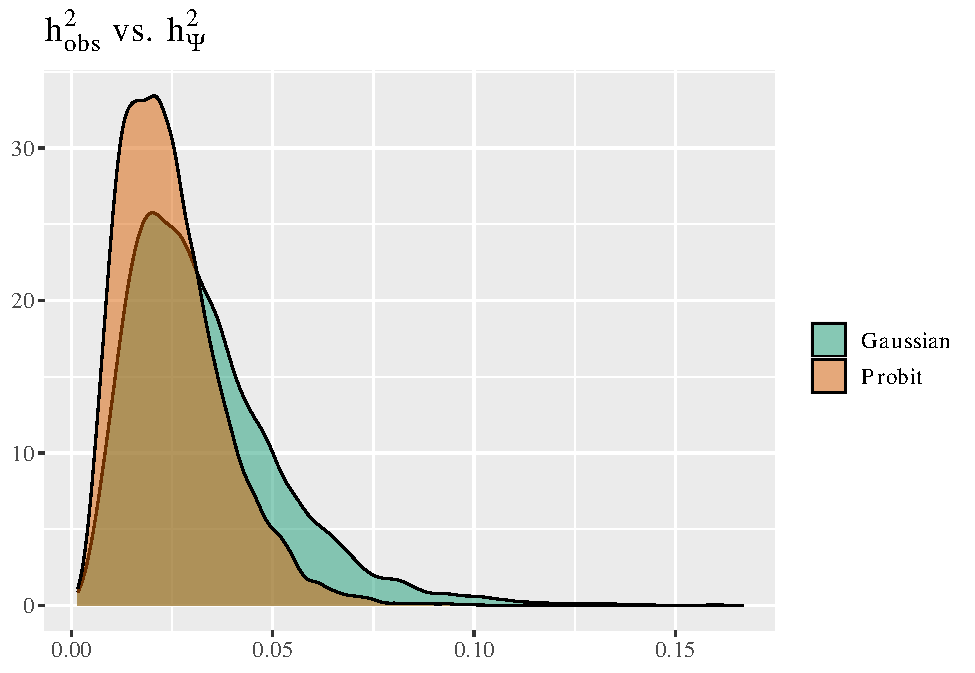
\includegraphics{figures/heritability_application_obsscale.pdf}
        \label{fig:posterior application heritability:observation}
    \end{subfigure}
    \caption[Heritability density for application data]{Posterior liability- and observation-scale densities of heritability for the application data.}
    \label{fig:posterior application heritability}
\end{figure}


\begin{figure}
    \centering
        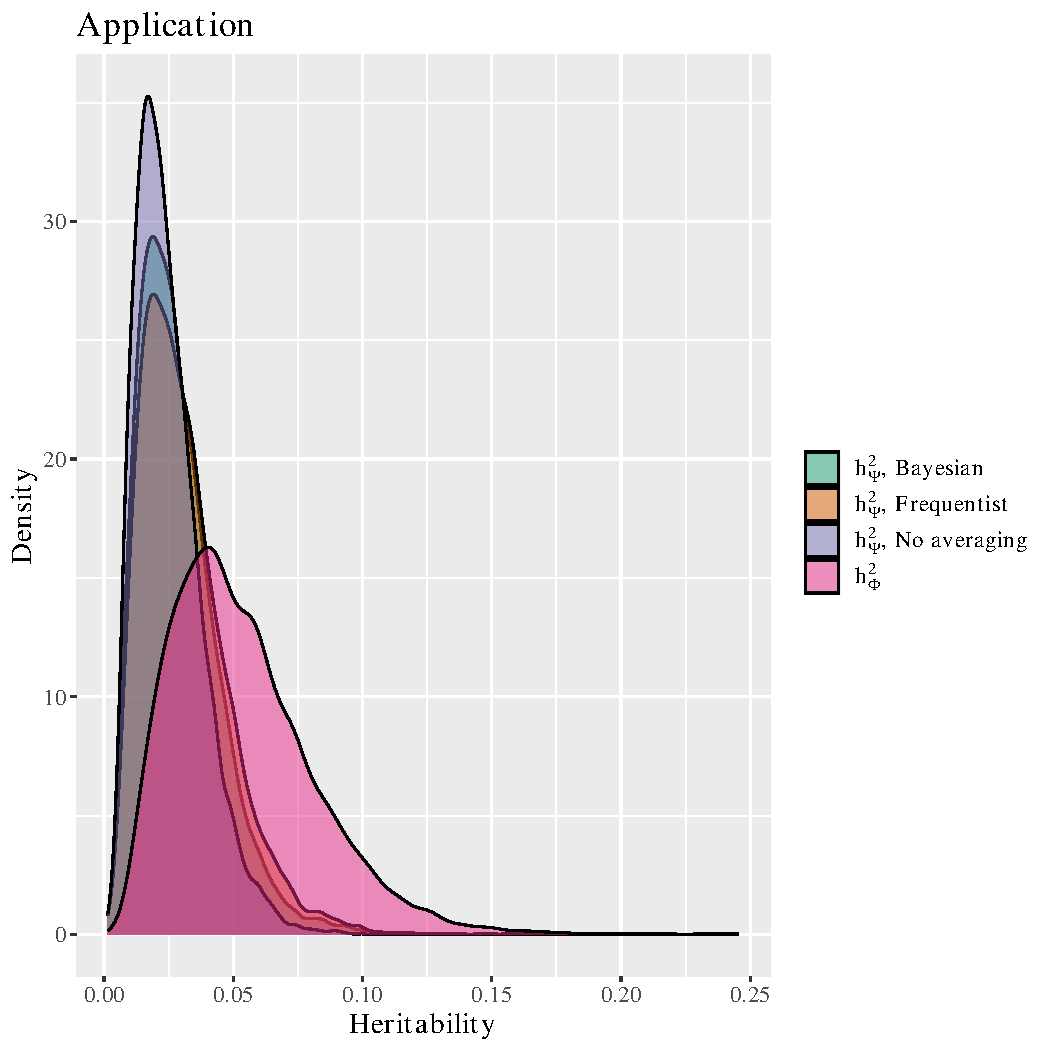
\includegraphics[width=0.8\textwidth]{figures/qgglmm-comparison-application.pdf}       
    \caption[$h^2_\Psi$ on application data, with varying parameter settings]{Estimated posterior heritability for the different back-transformations techniques, for a binomial probit model to the application data.}
    \label{fig:qgglmm application}
\end{figure}
\subsection{Gaussian residual analysis}
In addition to computing the estimated heritability, we would like to explore the residual distribution of the Gaussian model for the application dataset. We fit a Gaussian model using INLA to the application data, in which we also compute the model's PIT values to evaluate the goodness of fit. \autoref{fig:sorted pit values} shows the sorted PIT values in ascending order relative to their quantiles, which would resemble a straight line for a uniform distribution, which is not the case for our data. \autoref{fig:gaussian pit vs fitted} shows the PIT values over the mean of the posterior fitted values, as well as a cubic spline smoothing plot. The PIT values show a clear pattern rather than being uniformly distributed, which is also the case for the plot of the residuals (\autoref{fig:gaussian residuals}).
% In a well-fitted model, there should not be any clear pattern in the distribution.
% \todo{Should I make similar plots for a simulation dataset?}

Another result that we may attribute to the residuals of the Gaussian model is that INLA seems to not always converge for the first initial values for this dataset, but succeeds all times on its second attempt. We cannot observe the same errors when fitting probit models, nor in the Gaussian simulation case. It is also relevant to report the deviance information criteria for the Gaussian and corresponding probit model (\autoref{tab:application DICs}).

The final plot provided, \autoref{fig:relatedness offdiagonal}, is a general comparison of off-diagonal values in the relatedness matrix for both datasets. The figure showcases a relatively similar structure in both the simulation and the song sparrow data. In particular, the general relatedness in the song sparrow dataset has more tailing for larger values and a larger mode than in the simulation case. However, both datasets still provide off-diagonal relatedness values around the same area, $(0,0.2)$, strengthening the simulated data as a viable tool for interpreting real-world data.

% <<<<< DIC (Deviance Information criterion)
\begin{table}
    \centering
    \begin{tabular}{@{}ll@{}}
    \toprule
        Model           & DIC (Application data) \\ \midrule
        Binomial probit & 2600.499  \\
        Gaussian        & 2712.749 \\
        \bottomrule
    \end{tabular}
    \caption[DIC for application data]{Deviance information criteria (DIC) for the two model fits, for the application data. }
    \label{tab:application DICs}
\end{table}
% >>>>> DIC (Deviance Information criterion)

\begin{figure}
    \centering
    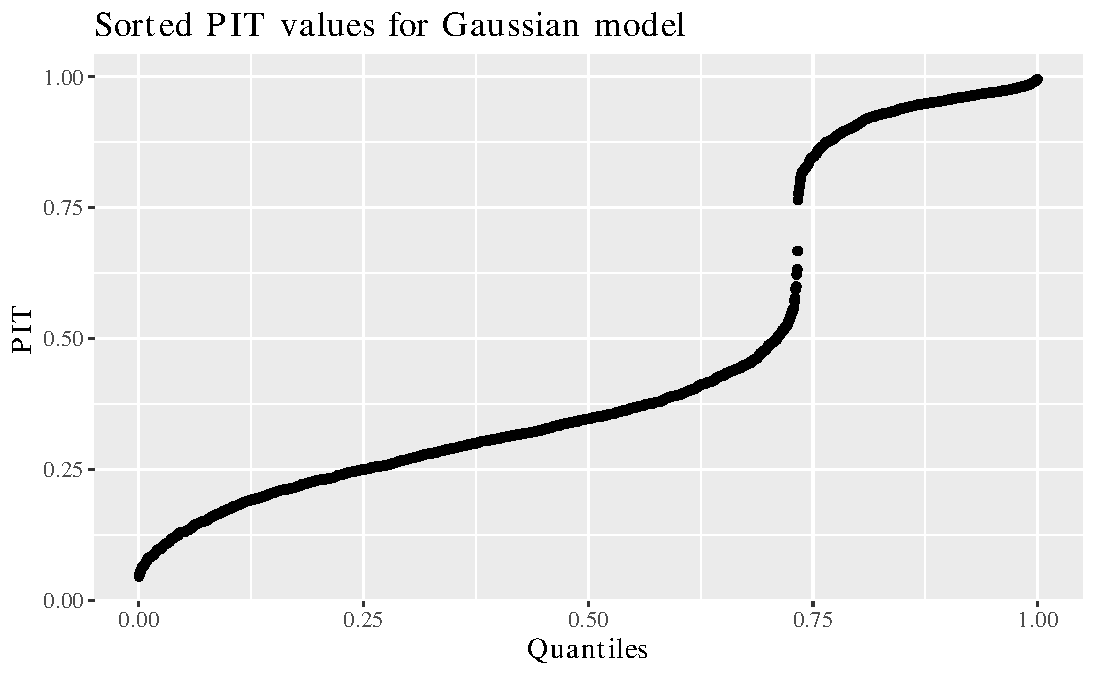
\includegraphics[width=0.8\textwidth]{figures/PIT-sorted.pdf}
    \caption{Sorted PIT values over quantiles in Gaussian application model.}
    \label{fig:sorted pit values}
\end{figure}

\begin{figure}
    \centering
    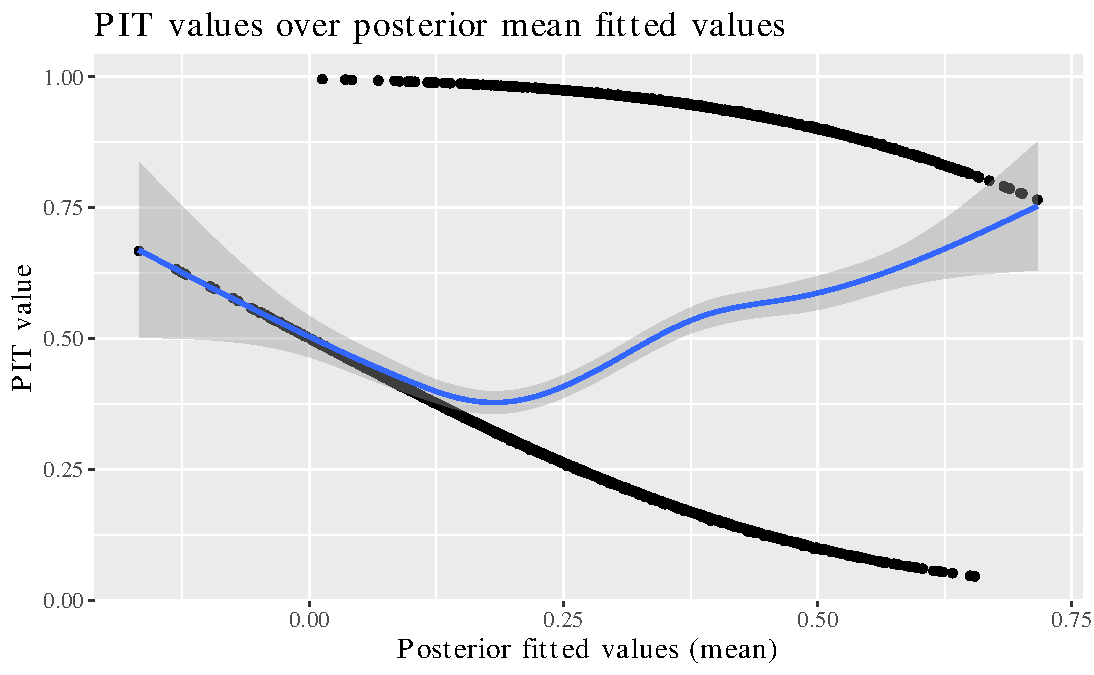
\includegraphics[width=0.8\textwidth]{figures/PIT-over-fitted.pdf}
    \caption[Gaussian model PIT vs fitted values in application]{PIT values over the mean of the posterior fitted values, using application data. The black dots are the PIT values, the blue line is a cubic spline smoothing and the grey area shows its 95\% confidence interval.}
    \label{fig:gaussian pit vs fitted}
\end{figure}

\begin{figure}
    \centering
    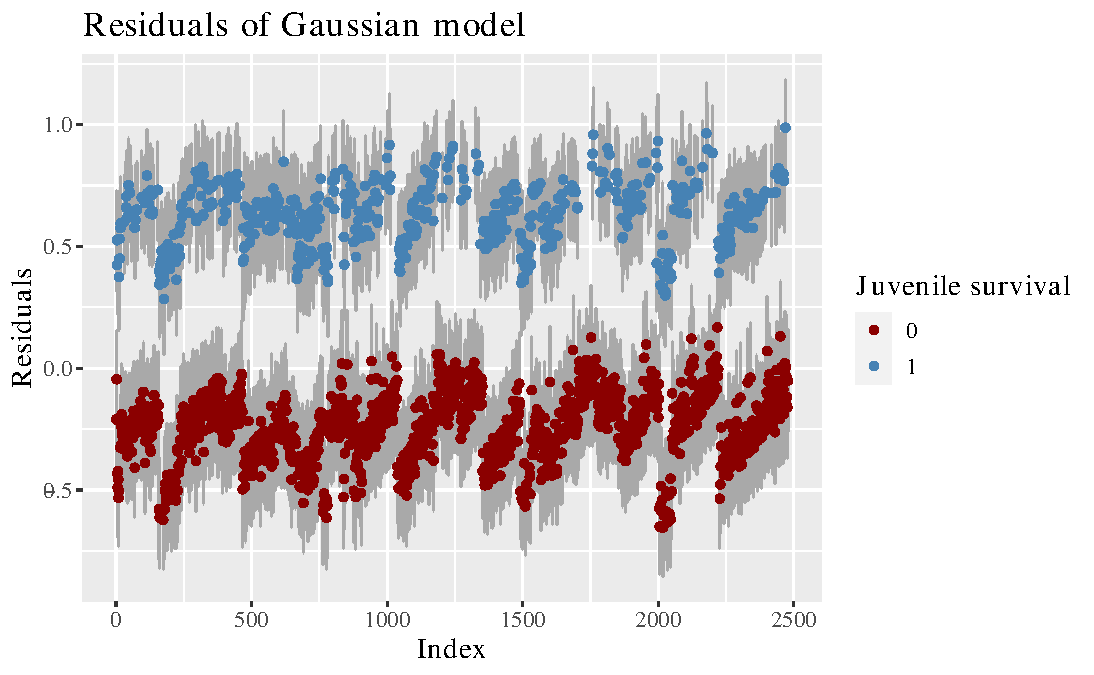
\includegraphics[width=0.8\textwidth]{figures/Residuals-gaussian.pdf}
    \caption[Residuals in Gaussian model, using simulation data]{Residuals of the Gaussian model with the song sparrow data. That is, $y_i-\hat y_i$ for all observed $i$. The blue-colored dots resemble the difference between the mean of the fitted values and the true observation where juvenile survival is true. Similarly, the red dots are when the trait is false (not survived). The dark grey lines are the 95\% credible intervals for each of the residuals, based on the quantiles computes from the posterior fitted values.}
    \label{fig:gaussian residuals}
\end{figure}

\begin{figure}
  \centering
  \begin{subfigure}[b]{0.5\textwidth}
    \centering
    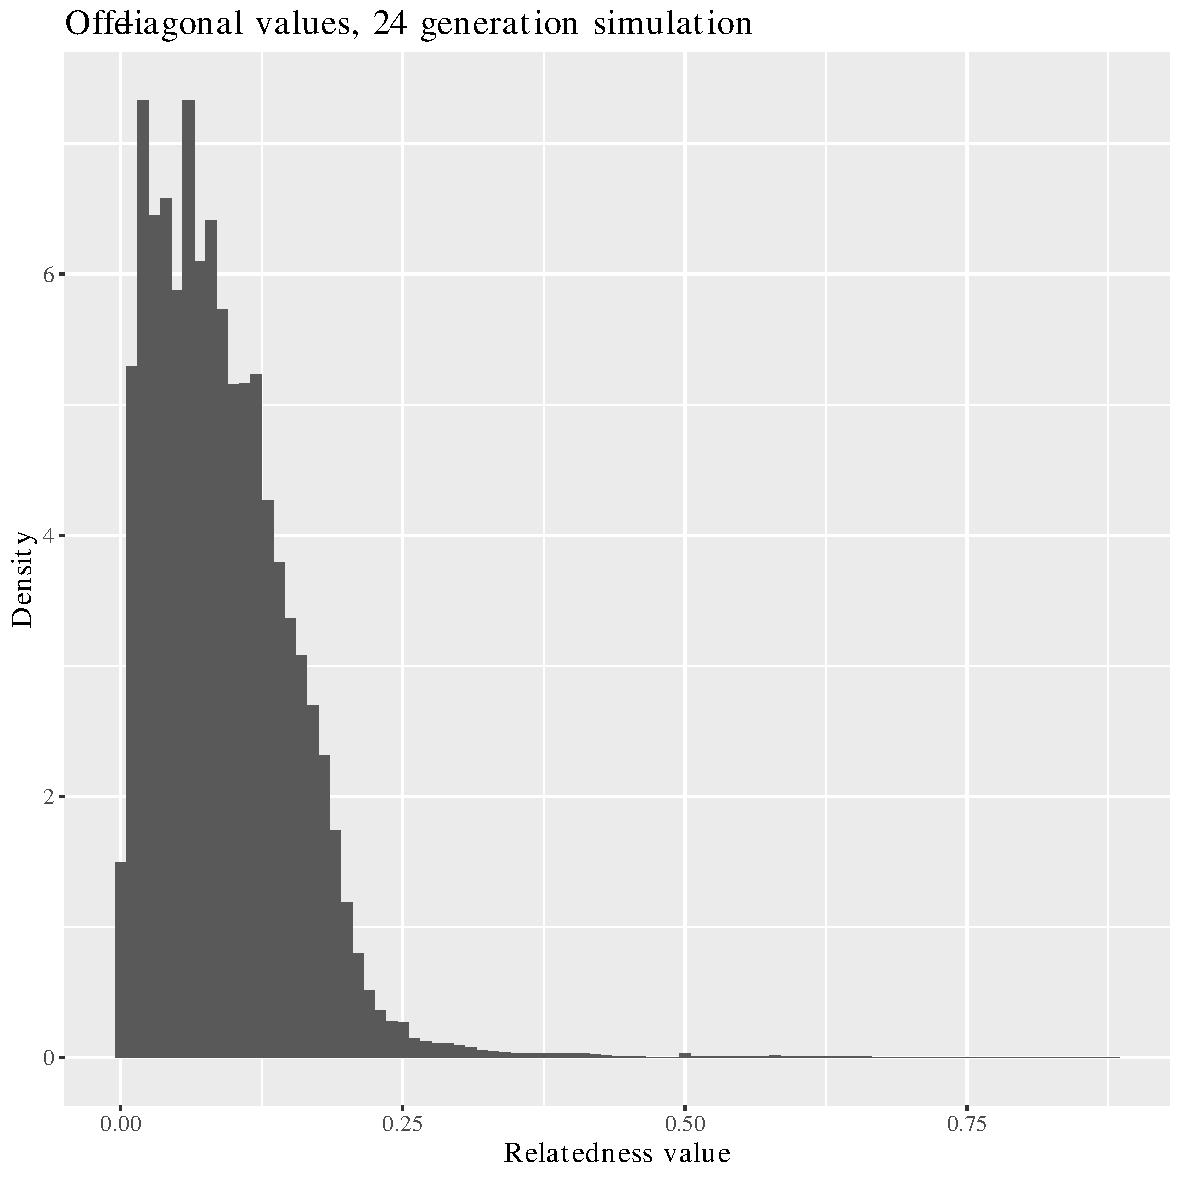
\includegraphics[width=\textwidth]{figures/relatedness-offdiagonal-sim.pdf}
    \caption{Simulation data}
    \label{fig:relatedness:simulation}
  \end{subfigure}%
  \begin{subfigure}[b]{0.5\textwidth}
    \centering
    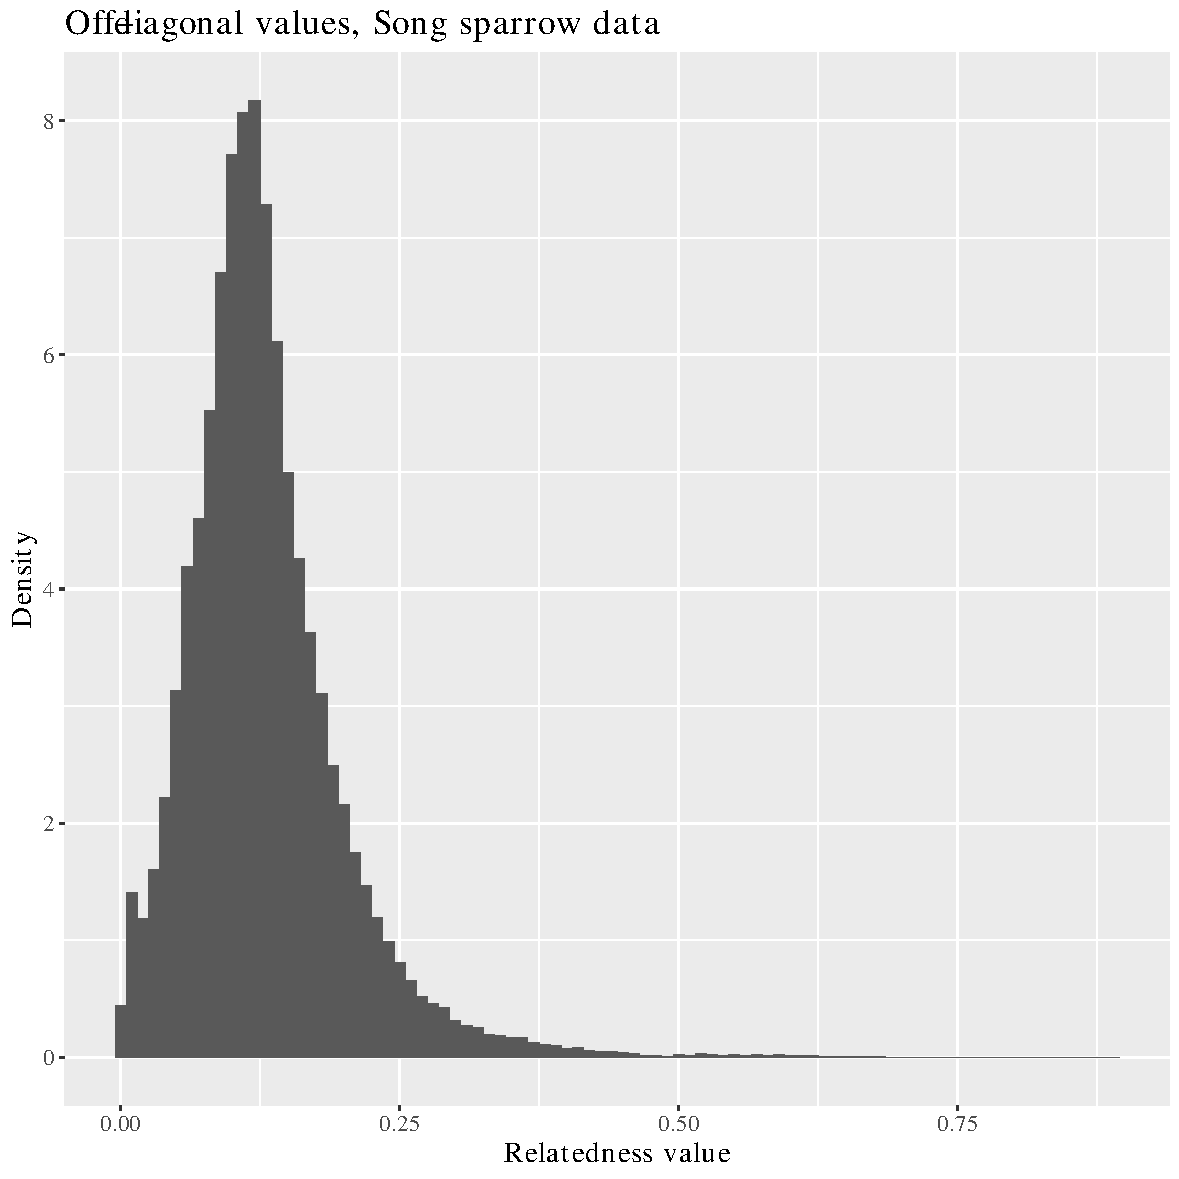
\includegraphics[width=\textwidth]{figures/relatedness-offdiagonal-songsparrow.pdf}
    \caption{Song Sparrow data}
    \label{fig:relatedness:realdata}
  \end{subfigure}
  \caption[Off-diagonal values in simulated relatedness matrix]{Histograms showing the density of the different relatedness values in the relatedness matrix for the simulation data, and the song sparrow data, respectively. The diagonal values (measuring relatedness to the individual itself) are not included, as self-relatedness is one by construction.}
  \label{fig:relatedness offdiagonal}
\end{figure}